\documentclass[a4paper,11pt]{report}
\usepackage[utf8]{inputenc}
\usepackage[english]{babel}
\usepackage[hyphens]{xurl}
\usepackage{csquotes}
\usepackage{pgfplots}
\usepackage[hidelinks]{hyperref}
\usepackage[backend=bibtex,urldate=iso]{biblatex}


\newenvironment{itquote}
	{\begin{quote}\itshape}
	{\end{quote}\ignorespacesafterend}

\pgfplotsset{compat=1.18}

\addbibresource{references.bib}


\title{Automatic Detection of common Incorrect Statements in Speeches of Swiss Politicians}
\author{Lena Merkli}

\begin{document}
	\maketitle
	
	\begin{abstract}
		Swiss politicians lie~\cite{SRF2022MachtWahrheit}.
		And they mostly get away with it~\cite{Hirstein2023}.
		\enquote{One reason for this is that fact checks, which can only be carried out retrospectively, are surprisingly ineffective. Listeners still remember the false information. The correction is forgotten.} -- Philipp Gerlach~\cite{SRF2022MachtWahrheit}.
		This technical report provides a comprehensive overview of the artificial intelligence components of the PolitScanner project.
		It aims to automatically detect false narratives and fake news in the speeches of Swiss politicians while avoiding the inaccuracies inherent in Large Language Models.
		\\\\
		All code can be found on GitHub~\url{https://github.com/lenamerkli/PolitScanner}.
		An inference-only example is available at~\url{https://huggingface.co/lenamerkli/PolitScanner}.
		\\\\
		This is an entry for the Swiss AI Challenge 2025.
		More information can be found at~\url{https://www.ki-challenge.ch/}.
	\end{abstract}

	\tableofcontents

	\chapter{System Architecture}\label{ch:system-architecture}

		\section{Database}\label{sec:database}
			At the core sits a vector database that stores facts and sentences talking about the topics relevant to these facts.
	    	These facts are available in a human-readable format at~\url{https://github.com/lenamerkli/PolitScanner/tree/main/data/raw}.
	    	ChromaDB has been chosen as it is a high performance vector database that is straightforward to use and has excellent python integration~\cite{chromadb}.

		\section{Inference Pipeline}\label{sec:inference-pipeline}
			A speech is split into sentences using a custom sentence splitter.
	    	These sentences are then grouped into overlapping chunks to provide context.
	    	Each chunk is used to query the vector database for relevant topics.
	    	A fine-tuned large language model checks if the topics are relevant to the statements in the chunk.

	    \section{Avoiding Large Language Model Inaccuracies}\label{sec:avoiding-large-language-model-inaccuracies}
			Large Language Models and other machine learning technologies are exclusively used to find the relevant facts.
            They have no influence on the presented facts.
	        Letting incorrect statements pass without detection is the worst that any machine learning based approach can do.
			An exception to this is the sentence splitter that could alter the meaning of the provided speech.
	        But as the sentence splitter iteratively improves python code, this would be transparent to the developers and users.

	    \section{Data Collection and Annotation}\label{sec:data-collection-and-annotation}
			All datasets in the PolitScanner project were annotated by a human.
			Facts were collected by researching on the internet biased by the developers.
			The dataset containing the facts has only 23 entries; enough for a proof-of-concept but way too little for a real-world application.
            The base texts to train the sentence splitter stem from the Swiss Parliament website~\cite{parliamentCH}.
	        To train the main model, speeches from the parliamentary website along with news articles (primarily interviews) were used for the base texts and annotated by the developers.

	\chapter{Training}\label{ch:training}
		\section{Sentence Splitter}\label{sec:sentence-splitter}
	        In each iteration, an input is provided to the current version and an assert-check is performed.
	        Any resulting errors are given to a local Large Language Model alongside the input, the expected output and the actual output, if available.
	        The model is given the task to improve the core functionality of the sentence splitter.
	        Our testing has shown, that the model should be larger than 20 billion parameters (dense) for acceptable results.

	    \section{Main Model}\label{sec:main-model}
	        The main model is a fine-tuned version of \enquote{Qwen3-1.7B}~\cite{qwen3}.
	        This choice has been made due to the following reasons:
	        \begin{itemize}
	        	\item It is a good and modern Large Language Model
				\item Downloading the model is possible
				\item Qwen3 is available in different sizes~\cite{qwen3}
	        	\item All its sizes are compatible with bits-and-bytes~\cite{dettmers20228bitoptimizersblockwisequantization}\cite{dettmers2023qloraefficientfinetuningquantized}
				\item Both UnslothAI and llama.cpp support Qwen3~\cite{unsloth}\cite{llamacpp}
	        \end{itemize}
	        One drawback of this selection is the Chinese censorship present in the models~\cite{lin2024chinese}
	        \begin{figure}[htbp]
	        	\centering
	        	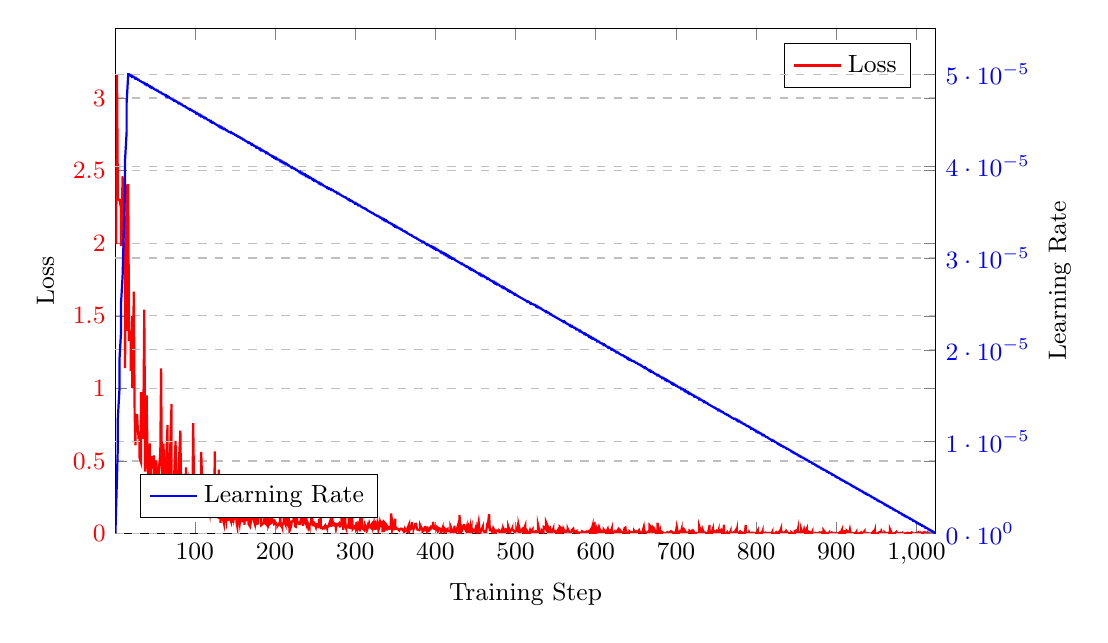
\begin{tikzpicture}
	        		\begin{axis}[
	        			width=12cm,
	        			height=8cm,
	        			xlabel={Training Step},
	        			ylabel={Loss},
	        			xmin=1, xmax=1024,
	        			ymin=0,
	        			legend pos=north east,
	        			ymajorgrids=true,
	        			grid style=dashed,
	        			scaled y ticks=false,
	        			tick label style={/pgf/number format/fixed},
	        			legend style={font=\small},
	        			label style={font=\small},
	        			tick label style={font=\small},
	        			y tick label style={color=red}
	        			]

	        			\addplot[
	        			color=red,
	        			mark=none,
	        			thick
	        			]
	        			coordinates {
	        				(1,2.4529)
	        				(2,1.9934)
	        				(3,3.1641)
	        				(4,2.3863)
	        				(4,2.3078)
	        				(6,2.2954)
	        				(6,2.3045)
	        				(8,2.2383)
	        				(8,1.9795)
	        				(10,2.4614)
	        				(11,1.9916)
	        				(12,1.9498)
	        				(13,1.9572)
	        				(13,1.1398)
	        				(15,2.4051)
	        				(15,1.3966)
	        				(17,2.4071)
	        				(18,1.3256)
	        				(19,1.3794)
	        				(20,1.3614)
	        				(20,1.1208)
	        				(22,1.4971)
	        				(22,1.0041)
	        				(24,1.6657)
	        				(25,0.822)
	        				(26,0.6082)
	        				(26,0.7115)
	        				(28,0.8243)
	        				(29,0.7174)
	        				(30,0.6531)
	        				(31,0.7033)
	        				(31,0.5239)
	        				(33,0.4896)
	        				(33,0.9744)
	        				(35,0.6529)
	        				(36,0.8837)
	        				(37,1.5431)
	        				(38,0.6987)
	        				(38,0.4275)
	        				(40,0.9518)
	        				(40,0.9031)
	        				(42,0.2577)
	        				(43,0.517)
	        				(44,0.6218)
	        				(44,0.1361)
	        				(46,0.5337)
	        				(46,0.477)
	        				(48,0.4569)
	        				(49,0.5393)
	        				(49,0.4188)
	        				(51,0.4195)
	        				(52,0.5045)
	        				(53,0.3815)
	        				(54,0.3007)
	        				(55,0.2926)
	        				(55,0.4309)
	        				(57,0.5578)
	        				(58,1.1373)
	        				(59,0.3758)
	        				(59,0.3984)
	        				(61,0.6192)
	        				(62,0.3701)
	        				(63,0.3292)
	        				(64,0.2303)
	        				(64,0.4474)
	        				(66,0.7487)
	        				(66,0.1717)
	        				(68,0.3512)
	        				(69,0.2364)
	        				(69,0.5168)
	        				(71,0.8925)
	        				(71,0.3878)
	        				(73,0.2851)
	        				(74,0.2109)
	        				(74,0.3656)
	        				(76,0.6384)
	        				(77,0.3685)
	        				(78,0.2615)
	        				(79,0.1956)
	        				(80,0.4796)
	        				(80,0.4728)
	        				(82,0.7087)
	        				(83,0.2754)
	        				(84,0.3486)
	        				(85,0.3538)
	        				(85,0.2905)
	        				(87,0.2431)
	        				(88,0.1838)
	        				(89,0.4555)
	        				(89,0.3387)
	        				(91,0.376)
	        				(91,0.2174)
	        				(93,0.1504)
	        				(94,0.3163)
	        				(94,0.2766)
	        				(96,0.2711)
	        				(97,0.2066)
	        				(98,0.7607)
	        				(99,0.3656)
	        				(100,0.247)
	        				(101,0.2375)
	        				(102,0.2392)
	        				(102,0.1289)
	        				(104,0.1213)
	        				(105,0.1957)
	        				(106,0.1604)
	        				(106,0.1355)
	        				(108,0.2749)
	        				(108,0.563)
	        				(110,0.2142)
	        				(111,0.2406)
	        				(112,0.184)
	        				(112,0.1971)
	        				(114,0.2068)
	        				(115,0.1623)
	        				(115,0.2167)
	        				(117,0.1107)
	        				(118,0.1959)
	        				(119,0.1475)
	        				(120,0.207)
	        				(120,0.2086)
	        				(122,0.118)
	        				(122,0.1396)
	        				(124,0.1717)
	        				(125,0.5669)
	        				(125,0.2662)
	        				(127,0.2963)
	        				(127,0.1611)
	        				(129,0.1368)
	        				(130,0.4402)
	        				(130,0.1087)
	        				(132,0.1116)
	        				(132,0.0741)
	        				(134,0.2752)
	        				(134,0.1238)
	        				(136,0.0774)
	        				(136,0.3626)
	        				(138,0.1119)
	        				(139,0.0844)
	        				(140,0.1786)
	        				(141,0.0863)
	        				(141,0.0893)
	        				(143,0.1867)
	        				(143,0.1157)
	        				(145,0.085)
	        				(145,0.0889)
	        				(147,0.0839)
	        				(148,0.2261)
	        				(149,0.1109)
	        				(150,0.139)
	        				(151,0.4012)
	        				(152,0.0774)
	        				(153,0.0476)
	        				(154,0.3458)
	        				(155,0.1015)
	        				(156,0.0665)
	        				(157,0.1113)
	        				(158,0.1446)
	        				(159,0.0849)
	        				(160,0.0854)
	        				(161,0.1539)
	        				(162,0.0596)
	        				(162,0.0867)
	        				(164,0.0919)
	        				(164,0.1082)
	        				(166,0.1636)
	        				(167,0.0972)
	        				(167,0.0664)
	        				(169,0.0488)
	        				(170,0.0838)
	        				(171,0.1646)
	        				(171,0.3407)
	        				(173,0.1032)
	        				(174,0.0836)
	        				(174,0.2294)
	        				(176,0.0826)
	        				(177,0.114)
	        				(177,0.0669)
	        				(179,0.0704)
	        				(180,0.1593)
	        				(181,0.2335)
	        				(181,0.1343)
	        				(183,0.1091)
	        				(183,0.0592)
	        				(185,0.0687)
	        				(186,0.0716)
	        				(187,0.1124)
	        				(188,0.0712)
	        				(189,0.0649)
	        				(189,0.1339)
	        				(191,0.1353)
	        				(192,0.0759)
	        				(192,0.058)
	        				(194,0.0866)
	        				(194,0.0683)
	        				(196,0.0754)
	        				(197,0.2008)
	        				(197,0.0838)
	        				(199,0.0887)
	        				(199,0.0638)
	        				(201,0.0668)
	        				(201,0.0737)
	        				(203,0.0548)
	        				(203,0.0517)
	        				(205,0.069)
	        				(206,0.0621)
	        				(207,0.2079)
	        				(207,0.0779)
	        				(209,0.0437)
	        				(209,0.0518)
	        				(211,0.084)
	        				(211,0.0917)
	        				(213,0.0644)
	        				(213,0.1634)
	        				(215,0.0658)
	        				(216,0.0579)
	        				(217,0.1104)
	        				(218,0.0702)
	        				(218,0.0165)
	        				(220,0.0485)
	        				(221,0.0838)
	        				(221,0.0844)
	        				(223,0.0847)
	        				(224,0.1794)
	        				(225,0.0503)
	        				(226,0.0475)
	        				(227,0.1334)
	        				(228,0.0723)
	        				(228,0.0829)
	        				(230,0.0663)
	        				(231,0.0661)
	        				(231,0.0601)
	        				(233,0.1283)
	        				(233,0.1459)
	        				(235,0.0532)
	        				(235,0.0636)
	        				(237,0.0821)
	        				(237,0.0974)
	        				(239,0.0637)
	        				(239,0.1017)
	        				(241,0.0617)
	        				(241,0.0712)
	        				(243,0.0428)
	        				(243,0.0578)
	        				(245,0.0732)
	        				(246,0.179)
	        				(247,0.0497)
	        				(247,0.0793)
	        				(249,0.0768)
	        				(249,0.0714)
	        				(251,0.0421)
	        				(252,0.0714)
	        				(252,0.0608)
	        				(254,0.0467)
	        				(255,0.0545)
	        				(255,0.0942)
	        				(257,0.1011)
	        				(257,0.0389)
	        				(259,0.0419)
	        				(260,0.0421)
	        				(260,0.0409)
	        				(262,0.0529)
	        				(262,0.039)
	        				(264,0.0492)
	        				(265,0.0343)
	        				(265,0.0442)
	        				(267,0.0503)
	        				(267,0.0587)
	        				(269,0.091)
	        				(270,0.0466)
	        				(270,0.1498)
	        				(272,0.0816)
	        				(273,0.0504)
	        				(273,0.0749)
	        				(275,0.0662)
	        				(276,0.0328)
	        				(277,0.0655)
	        				(278,0.0659)
	        				(278,0.0598)
	        				(280,0.0707)
	        				(281,0.0427)
	        				(281,0.0471)
	        				(283,0.0738)
	        				(283,0.123)
	        				(285,0.0423)
	        				(285,0.026)
	        				(287,0.1737)
	        				(288,0.0469)
	        				(289,0.0323)
	        				(289,0.055)
	        				(291,0.0466)
	        				(292,0.0714)
	        				(292,0.1913)
	        				(294,0.0307)
	        				(294,0.0378)
	        				(296,0.1433)
	        				(297,0.034)
	        				(297,0.0325)
	        				(299,0.0472)
	        				(300,0.0376)
	        				(300,0.0484)
	        				(302,0.0685)
	        				(303,0.0325)
	        				(304,0.053)
	        				(304,0.0487)
	        				(306,0.0257)
	        				(307,0.0374)
	        				(307,0.1863)
	        				(309,0.0297)
	        				(309,0.0365)
	        				(311,0.0258)
	        				(312,0.0628)
	        				(313,0.0474)
	        				(314,0.0225)
	        				(315,0.0418)
	        				(315,0.0278)
	        				(317,0.0579)
	        				(317,0.0534)
	        				(319,0.0431)
	        				(319,0.0513)
	        				(321,0.0685)
	        				(322,0.0379)
	        				(323,0.064)
	        				(323,0.0575)
	        				(325,0.0747)
	        				(325,0.0338)
	        				(327,0.0348)
	        				(328,0.067)
	        				(329,0.0234)
	        				(330,0.0407)
	        				(331,0.0805)
	        				(332,0.0589)
	        				(333,0.0515)
	        				(334,0.0889)
	        				(334,0.017)
	        				(336,0.019)
	        				(336,0.0794)
	        				(338,0.0672)
	        				(338,0.0275)
	        				(340,0.0279)
	        				(341,0.0365)
	        				(341,0.0461)
	        				(343,0.0343)
	        				(344,0.0358)
	        				(345,0.1388)
	        				(346,0.0288)
	        				(347,0.0612)
	        				(348,0.0224)
	        				(348,0.0374)
	        				(350,0.1018)
	        				(350,0.0321)
	        				(352,0.0342)
	        				(352,0.0371)
	        				(354,0.0272)
	        				(355,0.0211)
	        				(356,0.0312)
	        				(357,0.0347)
	        				(358,0.0339)
	        				(359,0.0298)
	        				(359,0.0287)
	        				(361,0.0107)
	        				(362,0.0327)
	        				(363,0.0182)
	        				(364,0.0169)
	        				(365,0.0136)
	        				(365,0.0334)
	        				(367,0.0606)
	        				(367,0.0119)
	        				(369,0.0423)
	        				(370,0.0433)
	        				(371,0.0807)
	        				(371,0.0378)
	        				(373,0.0458)
	        				(373,0.0333)
	        				(375,0.0662)
	        				(376,0.067)
	        				(377,0.0358)
	        				(377,0.0296)
	        				(379,0.0248)
	        				(379,0.0254)
	        				(381,0.0281)
	        				(381,0.0597)
	        				(383,0.0353)
	        				(384,0.0336)
	        				(384,0.0135)
	        				(386,0.0223)
	        				(387,0.0526)
	        				(387,0.0393)
	        				(389,0.0214)
	        				(390,0.0489)
	        				(390,0.0169)
	        				(392,0.0308)
	        				(393,0.0378)
	        				(393,0.0277)
	        				(395,0.0432)
	        				(395,0.0357)
	        				(397,0.0445)
	        				(397,0.0812)
	        				(399,0.0261)
	        				(399,0.0311)
	        				(401,0.043)
	        				(401,0.0373)
	        				(403,0.014)
	        				(404,0.031)
	        				(404,0.039)
	        				(406,0.0334)
	        				(407,0.0244)
	        				(407,0.0062)
	        				(409,0.0381)
	        				(409,0.0234)
	        				(411,0.013)
	        				(411,0.0382)
	        				(413,0.023)
	        				(413,0.0237)
	        				(415,0.0315)
	        				(415,0.0193)
	        				(417,0.0193)
	        				(417,0.0161)
	        				(419,0.0131)
	        				(419,0.0482)
	        				(421,0.0193)
	        				(421,0.0072)
	        				(423,0.0189)
	        				(424,0.0543)
	        				(424,0.0168)
	        				(426,0.0279)
	        				(426,0.0124)
	        				(428,0.0533)
	        				(428,0.0405)
	        				(430,0.0032)
	        				(430,0.1284)
	        				(432,0.0105)
	        				(433,0.0165)
	        				(433,0.051)
	        				(435,0.0381)
	        				(436,0.0657)
	        				(436,0.0489)
	        				(438,0.0227)
	        				(439,0.0432)
	        				(439,0.0134)
	        				(441,0.0471)
	        				(442,0.0105)
	        				(443,0.037)
	        				(443,0.0087)
	        				(445,0.044)
	        				(445,0.0035)
	        				(447,0.0243)
	        				(448,0.0159)
	        				(449,0.015)
	        				(450,0.0331)
	        				(450,0.0128)
	        				(452,0.0073)
	        				(452,0.0175)
	        				(454,0.0804)
	        				(455,0.0209)
	        				(455,0.0177)
	        				(457,0.0275)
	        				(457,0.0187)
	        				(459,0.0462)
	        				(459,0.0312)
	        				(461,0.0114)
	        				(462,0.0137)
	        				(463,0.0048)
	        				(464,0.0389)
	        				(465,0.0755)
	        				(465,0.0367)
	        				(467,0.1351)
	        				(468,0.0162)
	        				(468,0.0397)
	        				(470,0.0192)
	        				(471,0.0123)
	        				(472,0.0343)
	        				(473,0.0174)
	        				(473,0.0298)
	        				(475,0.0085)
	        				(475,0.0222)
	        				(477,0.0219)
	        				(477,0.0166)
	        				(479,0.0193)
	        				(480,0.0078)
	        				(480,0.0191)
	        				(482,0.0065)
	        				(483,0.0229)
	        				(483,0.0081)
	        				(485,0.0056)
	        				(485,0.032)
	        				(487,0.0046)
	        				(488,0.0278)
	        				(489,0.0235)
	        				(490,0.0308)
	        				(491,0.0013)
	        				(491,0.0485)
	        				(493,0.0162)
	        				(493,0.0266)
	        				(495,0.0233)
	        				(496,0.0372)
	        				(496,0.029)
	        				(498,0.0208)
	        				(499,0.008)
	        				(499,0.0136)
	        				(501,0.0178)
	        				(502,0.0404)
	        				(502,0.0197)
	        				(504,0.012)
	        				(504,0.0544)
	        				(506,0.0041)
	        				(506,0.0166)
	        				(508,0.0279)
	        				(508,0.0243)
	        				(510,0.0083)
	        				(510,0.0247)
	        				(512,0.0542)
	        				(512,0.0058)
	        				(514,0.0217)
	        				(515,0.0078)
	        				(515,0.0038)
	        				(517,0.0028)
	        				(518,0.0227)
	        				(519,0.0045)
	        				(519,0.0122)
	        				(521,0.0283)
	        				(521,0.0123)
	        				(523,0.0115)
	        				(524,0.0103)
	        				(525,0.017)
	        				(526,0.0147)
	        				(526,0.0121)
	        				(528,0.0122)
	        				(528,0.0612)
	        				(530,0.0132)
	        				(531,0.0095)
	        				(532,0.0073)
	        				(533,0.0113)
	        				(533,0.019)
	        				(535,0.0045)
	        				(535,0.046)
	        				(537,0.0391)
	        				(538,0.03)
	        				(538,0.0795)
	        				(540,0.0525)
	        				(541,0.0088)
	        				(542,0.0367)
	        				(543,0.0409)
	        				(544,0.0087)
	        				(545,0.0056)
	        				(545,0.0058)
	        				(547,0.0341)
	        				(547,0.0259)
	        				(549,0.0126)
	        				(549,0.0177)
	        				(551,0.0104)
	        				(551,0.0065)
	        				(553,0.0258)
	        				(553,0.0075)
	        				(555,0.0049)
	        				(555,0.049)
	        				(557,0.0381)
	        				(557,0.0071)
	        				(559,0.0101)
	        				(560,0.0217)
	        				(560,0.0296)
	        				(562,0.0075)
	        				(563,0.014)
	        				(563,0.0071)
	        				(565,0.0279)
	        				(565,0.0355)
	        				(567,0.0114)
	        				(568,0.0081)
	        				(568,0.0041)
	        				(570,0.015)
	        				(570,0.0234)
	        				(572,0.0345)
	        				(573,0.009)
	        				(574,0.0121)
	        				(575,0.0144)
	        				(576,0.0176)
	        				(576,0.0024)
	        				(578,0.0082)
	        				(579,0.0039)
	        				(580,0.0032)
	        				(580,0.0067)
	        				(582,0.0086)
	        				(583,0.0033)
	        				(583,0.0159)
	        				(585,0.0109)
	        				(586,0.0033)
	        				(586,0.0087)
	        				(588,0.0134)
	        				(588,0.0059)
	        				(590,0.006)
	        				(591,0.016)
	        				(592,0.0121)
	        				(592,0.013)
	        				(594,0.0309)
	        				(594,0.0101)
	        				(596,0.0522)
	        				(596,0.0116)
	        				(598,0.0493)
	        				(599,0.0062)
	        				(600,0.0082)
	        				(601,0.0359)
	        				(602,0.0199)
	        				(602,0.0041)
	        				(604,0.0461)
	        				(605,0.0283)
	        				(605,0.007)
	        				(607,0.0181)
	        				(608,0.0077)
	        				(609,0.0054)
	        				(610,0.0182)
	        				(610,0.0281)
	        				(612,0.0142)
	        				(613,9.00e-04)
	        				(613,0.0076)
	        				(615,0.0326)
	        				(616,0.0025)
	        				(616,0.0012)
	        				(618,0.0202)
	        				(619,0.0149)
	        				(620,0.0329)
	        				(620,0.0052)
	        				(622,0.0037)
	        				(623,0.0108)
	        				(623,0.0098)
	        				(625,0.0041)
	        				(626,0.0124)
	        				(626,0.0098)
	        				(628,0.0133)
	        				(629,0.0011)
	        				(629,0.0226)
	        				(631,0.0033)
	        				(631,0.0184)
	        				(633,0.0018)
	        				(634,0.0021)
	        				(635,0.0168)
	        				(636,0.0384)
	        				(637,0.042)
	        				(638,0.0013)
	        				(639,0.003)
	        				(640,0.0016)
	        				(640,0.0064)
	        				(642,0.0126)
	        				(642,0.016)
	        				(644,0.0076)
	        				(645,0.0029)
	        				(645,0.0104)
	        				(647,0.0068)
	        				(648,0.0057)
	        				(648,0.0193)
	        				(650,0.0032)
	        				(651,0.015)
	        				(652,0.0132)
	        				(652,0.0047)
	        				(654,0.0232)
	        				(655,0.0081)
	        				(656,0.0074)
	        				(657,0.0068)
	        				(658,0.0111)
	        				(658,0.0068)
	        				(660,0.0476)
	        				(661,0.0061)
	        				(661,0.0178)
	        				(663,0.0017)
	        				(664,0.0039)
	        				(664,0.0037)
	        				(666,0.0177)
	        				(667,0.0104)
	        				(667,0.0589)
	        				(669,0.0474)
	        				(669,0.0322)
	        				(671,0.001)
	        				(672,0.002)
	        				(672,0.0274)
	        				(674,0.0011)
	        				(674,0.0215)
	        				(676,0.0014)
	        				(677,0.0123)
	        				(677,0.0747)
	        				(679,0.0095)
	        				(680,0.0227)
	        				(680,0.0053)
	        				(682,0.0112)
	        				(683,0.0017)
	        				(683,0.0106)
	        				(685,0.0028)
	        				(686,0.0014)
	        				(687,0.0015)
	        				(687,0.0023)
	        				(689,0.0082)
	        				(689,0.0053)
	        				(691,0.0084)
	        				(692,0.0082)
	        				(693,0.013)
	        				(694,0.0037)
	        				(695,0.0037)
	        				(695,0.0127)
	        				(697,0.0054)
	        				(697,0.0043)
	        				(699,0.0068)
	        				(700,0.0122)
	        				(701,0.0482)
	        				(702,0.017)
	        				(702,0.0044)
	        				(704,0.0019)
	        				(705,0.0138)
	        				(706,0.0078)
	        				(707,0.0288)
	        				(707,0.0043)
	        				(709,0.0251)
	        				(710,0.0123)
	        				(711,0.0173)
	        				(711,0.0218)
	        				(713,0.0056)
	        				(713,0.001)
	        				(715,0.001)
	        				(715,0.0046)
	        				(717,0.0174)
	        				(717,0.0188)
	        				(719,0.0095)
	        				(720,0.0184)
	        				(721,0.0029)
	        				(722,0.0158)
	        				(723,0.006)
	        				(723,6.00e-04)
	        				(725,0.0018)
	        				(726,0.0048)
	        				(727,0.003)
	        				(728,6.00e-04)
	        				(729,9.00e-04)
	        				(729,0.0516)
	        				(731,0.0151)
	        				(732,0.0012)
	        				(733,0.0321)
	        				(734,0.0158)
	        				(735,0.0079)
	        				(735,0.004)
	        				(737,0.0075)
	        				(738,0.0023)
	        				(739,0.0028)
	        				(740,0.0049)
	        				(740,0.0013)
	        				(742,0.0596)
	        				(742,0.0053)
	        				(744,0.0038)
	        				(744,0.0016)
	        				(746,0.0335)
	        				(746,0.006)
	        				(748,0.0155)
	        				(749,0.0053)
	        				(750,0.0125)
	        				(750,0.0016)
	        				(752,4.00e-04)
	        				(753,0.0191)
	        				(753,0.0025)
	        				(755,0.0184)
	        				(756,0.001)
	        				(757,0.0178)
	        				(758,0.0025)
	        				(759,0.0138)
	        				(760,0.0608)
	        				(760,0.0036)
	        				(762,8.00e-04)
	        				(763,0.0013)
	        				(764,0.0112)
	        				(765,8.00e-04)
	        				(766,0.0037)
	        				(767,0.0029)
	        				(768,0.0164)
	        				(768,0.0025)
	        				(770,0.0055)
	        				(770,0.0024)
	        				(772,0.0087)
	        				(773,0.0015)
	        				(774,0.0161)
	        				(775,0.002)
	        				(776,0.027)
	        				(776,8.00e-04)
	        				(778,0.0021)
	        				(778,0.0027)
	        				(780,0.0153)
	        				(781,0.0071)
	        				(782,0.0095)
	        				(783,0.003)
	        				(783,0.0042)
	        				(785,0.0028)
	        				(786,0.005)
	        				(787,0.0593)
	        				(787,7.00e-04)
	        				(789,0.0032)
	        				(790,0.0011)
	        				(791,0.0131)
	        				(792,0.0021)
	        				(793,0.001)
	        				(794,0.0042)
	        				(794,0.0016)
	        				(796,0.0017)
	        				(797,0.0053)
	        				(798,0.0014)
	        				(799,0.001)
	        				(800,0.001)
	        				(800,0.0014)
	        				(802,0.0213)
	        				(802,0.0085)
	        				(804,9.00e-04)
	        				(805,0.0043)
	        				(806,0.0059)
	        				(807,0.0012)
	        				(808,0.0174)
	        				(808,0.012)
	        				(810,0.0047)
	        				(811,0.0062)
	        				(811,0.0022)
	        				(813,0.0018)
	        				(814,0.0047)
	        				(815,0.0051)
	        				(815,0.0031)
	        				(817,0.0038)
	        				(817,0.001)
	        				(819,7.00e-04)
	        				(820,0.0118)
	        				(820,0.0016)
	        				(822,6.00e-04)
	        				(823,0.001)
	        				(824,0.0015)
	        				(825,0.0094)
	        				(826,0.0014)
	        				(827,0.0048)
	        				(827,9.00e-04)
	        				(829,0.015)
	        				(829,0.0017)
	        				(831,0.0333)
	        				(831,0.0234)
	        				(833,0.0035)
	        				(834,7.00e-04)
	        				(834,0.0019)
	        				(836,0.0117)
	        				(837,0.0011)
	        				(838,0.0024)
	        				(838,0.0156)
	        				(840,0.0014)
	        				(841,0.0027)
	        				(842,0.0022)
	        				(843,0.0048)
	        				(844,0.0083)
	        				(844,0.0096)
	        				(846,4.00e-04)
	        				(846,0.0017)
	        				(848,2.00e-04)
	        				(848,0.0173)
	        				(850,0.0213)
	        				(851,0.0014)
	        				(852,0.0274)
	        				(852,0.0195)
	        				(854,5.00e-04)
	        				(854,0.0029)
	        				(856,0.0037)
	        				(856,0.0336)
	        				(858,7.00e-04)
	        				(859,0.0028)
	        				(860,0.0303)
	        				(861,0.0119)
	        				(861,0.0015)
	        				(863,0.0289)
	        				(863,0.0025)
	        				(865,0.0096)
	        				(866,6.00e-04)
	        				(866,0.0128)
	        				(868,0.0078)
	        				(869,0.0023)
	        				(870,0.0143)
	        				(870,0.0011)
	        				(872,0.0014)
	        				(873,0.0014)
	        				(874,0.0019)
	        				(874,0.0053)
	        				(876,0.0037)
	        				(876,5.00e-04)
	        				(878,0.0056)
	        				(878,6.00e-04)
	        				(880,0.007)
	        				(881,0.008)
	        				(881,0.0035)
	        				(883,0.0022)
	        				(884,0.0019)
	        				(884,0.0235)
	        				(886,0.0079)
	        				(887,0.0022)
	        				(888,0.0031)
	        				(888,0.0032)
	        				(890,5.00e-04)
	        				(891,0.0075)
	        				(891,3.00e-04)
	        				(893,0.0022)
	        				(894,0.0085)
	        				(895,0.0063)
	        				(895,0.0038)
	        				(897,0.0016)
	        				(898,0.0012)
	        				(899,8.00e-04)
	        				(899,0.004)
	        				(901,0.0013)
	        				(901,0.0013)
	        				(903,0.003)
	        				(904,0.0087)
	        				(905,0.0056)
	        				(905,0.0012)
	        				(907,0.0263)
	        				(907,6.00e-04)
	        				(909,0.002)
	        				(910,0.0162)
	        				(911,0.0139)
	        				(911,9.00e-04)
	        				(913,6.00e-04)
	        				(913,0.0198)
	        				(915,0.0084)
	        				(916,0.001)
	        				(917,0.0288)
	        				(918,8.00e-04)
	        				(918,7.00e-04)
	        				(920,0.0029)
	        				(920,0.0017)
	        				(922,0.0018)
	        				(922,9.00e-04)
	        				(924,0.0024)
	        				(925,0.0117)
	        				(925,4.00e-04)
	        				(927,3.00e-04)
	        				(928,0.0019)
	        				(929,0.0014)
	        				(929,0.001)
	        				(931,0.0089)
	        				(932,8.00e-04)
	        				(933,0.0015)
	        				(933,0.0018)
	        				(935,0.0159)
	        				(935,0.0012)
	        				(937,0.0013)
	        				(937,8.00e-04)
	        				(939,0.0019)
	        				(939,0.0032)
	        				(941,2.00e-04)
	        				(942,4.00e-04)
	        				(943,0.0015)
	        				(944,3.00e-04)
	        				(944,0.0019)
	        				(946,0.0138)
	        				(947,7.00e-04)
	        				(948,0.0196)
	        				(948,6.00e-04)
	        				(950,0.0013)
	        				(951,5.00e-04)
	        				(951,0.0019)
	        				(953,0.0074)
	        				(953,6.00e-04)
	        				(955,5.00e-04)
	        				(956,0.0171)
	        				(957,7.00e-04)
	        				(958,0.0012)
	        				(959,5.00e-04)
	        				(960,6.00e-04)
	        				(960,0.0106)
	        				(962,6.00e-04)
	        				(962,0.001)
	        				(964,0.004)
	        				(964,0.0028)
	        				(966,0.003)
	        				(967,0.0032)
	        				(967,0.0296)
	        				(969,0.0036)
	        				(970,6.00e-04)
	        				(971,8.00e-04)
	        				(971,0.0012)
	        				(973,0.0031)
	        				(973,0.0011)
	        				(975,0.0128)
	        				(976,0.0016)
	        				(977,0.003)
	        				(978,0.0014)
	        				(978,0.0013)
	        				(980,0.0049)
	        				(981,0.0011)
	        				(982,0.0047)
	        				(982,4.00e-04)
	        				(984,3.00e-04)
	        				(984,4.00e-04)
	        				(986,2.00e-04)
	        				(986,6.00e-04)
	        				(988,0.0043)
	        				(988,0.0037)
	        				(990,0.0043)
	        				(991,4.00e-04)
	        				(992,0.001)
	        				(992,0.0014)
	        				(994,0.0087)
	        				(995,7.00e-04)
	        				(996,4.00e-04)
	        				(996,0.0014)
	        				(998,0.001)
	        				(999,0.003)
	        				(1000,0.0015)
	        				(1000,5.00e-04)
	        				(1002,0.0083)
	        				(1002,4.00e-04)
	        				(1004,0.0058)
	        				(1004,8.00e-04)
	        				(1006,0.0033)
	        				(1007,7.00e-04)
	        				(1007,0.0049)
	        				(1009,0.0079)
	        				(1010,8.00e-04)
	        				(1011,0.0012)
	        				(1011,0.0078)
	        				(1013,0.0013)
	        				(1014,0.0082)
	        				(1015,0.002)
	        				(1015,0.0019)
	        				(1017,7.00e-04)
	        				(1017,7.00e-04)
	        				(1019,0.0017)
	        				(1020,4.00e-04)
	        				(1020,0.001)
	        				(1022,0.001)
	        				(1022,0.0012)
	        				(1024,5.00e-04)
	        			};
	        			\addlegendentry{Loss}
	        		\end{axis}
	        		\begin{axis}[
	        			width=12cm,
	        			height=8cm,
	        			xlabel={Training Step},
	        			ylabel={Learning Rate},
	        			xmin=1, xmax=1024,
	        			ymin=0,
	        			legend pos=south west,
	        			axis y line*=right,
	        			axis x line=none,
	        			ymajorgrids=true,
	        			grid style=dashed,
	        			scaled y ticks=false,
	        			y tick label style={/pgf/number format/sci},
	        			tick label style={/pgf/number format/fixed},
	        			legend style={font=\small},
	        			label style={font=\small},
	        			tick label style={font=\small},
	        			y tick label style={color=blue}
	        			]

	        			\addplot[
	        			color=blue,
	        			mark=none,
	        			thick
	        			]
	        			coordinates {
	        				(1,0)
	        				(2,3.13e-06)
	        				(3,6.25e-06)
	        				(4,9.38e-06)
	        				(4,1.25e-05)
	        				(6,1.56e-05)
	        				(6,1.88e-05)
	        				(8,2.19e-05)
	        				(8,2.50e-05)
	        				(10,2.81e-05)
	        				(11,3.13e-05)
	        				(12,3.44e-05)
	        				(13,3.75e-05)
	        				(13,4.06e-05)
	        				(15,4.37e-05)
	        				(15,4.69e-05)
	        				(17,5.00e-05)
	        				(18,5.00e-05)
	        				(19,4.99e-05)
	        				(20,4.99e-05)
	        				(20,4.98e-05)
	        				(22,4.98e-05)
	        				(22,4.97e-05)
	        				(24,4.97e-05)
	        				(25,4.96e-05)
	        				(26,4.96e-05)
	        				(26,4.95e-05)
	        				(28,4.95e-05)
	        				(29,4.94e-05)
	        				(30,4.94e-05)
	        				(31,4.93e-05)
	        				(31,4.93e-05)
	        				(33,4.92e-05)
	        				(33,4.92e-05)
	        				(35,4.91e-05)
	        				(36,4.91e-05)
	        				(37,4.90e-05)
	        				(38,4.90e-05)
	        				(38,4.89e-05)
	        				(40,4.89e-05)
	        				(40,4.88e-05)
	        				(42,4.88e-05)
	        				(43,4.87e-05)
	        				(44,4.87e-05)
	        				(44,4.86e-05)
	        				(46,4.86e-05)
	        				(46,4.85e-05)
	        				(48,4.85e-05)
	        				(49,4.84e-05)
	        				(49,4.84e-05)
	        				(51,4.83e-05)
	        				(52,4.83e-05)
	        				(53,4.82e-05)
	        				(54,4.82e-05)
	        				(55,4.81e-05)
	        				(55,4.81e-05)
	        				(57,4.80e-05)
	        				(58,4.80e-05)
	        				(59,4.79e-05)
	        				(59,4.79e-05)
	        				(61,4.78e-05)
	        				(62,4.78e-05)
	        				(63,4.77e-05)
	        				(64,4.77e-05)
	        				(64,4.76e-05)
	        				(66,4.76e-05)
	        				(66,4.75e-05)
	        				(68,4.75e-05)
	        				(69,4.74e-05)
	        				(69,4.74e-05)
	        				(71,4.73e-05)
	        				(71,4.73e-05)
	        				(73,4.72e-05)
	        				(74,4.72e-05)
	        				(74,4.71e-05)
	        				(76,4.71e-05)
	        				(77,4.70e-05)
	        				(78,4.70e-05)
	        				(79,4.69e-05)
	        				(80,4.69e-05)
	        				(80,4.68e-05)
	        				(82,4.68e-05)
	        				(83,4.67e-05)
	        				(84,4.67e-05)
	        				(85,4.66e-05)
	        				(85,4.66e-05)
	        				(87,4.65e-05)
	        				(88,4.65e-05)
	        				(89,4.64e-05)
	        				(89,4.64e-05)
	        				(91,4.63e-05)
	        				(91,4.63e-05)
	        				(93,4.62e-05)
	        				(94,4.62e-05)
	        				(94,4.61e-05)
	        				(96,4.61e-05)
	        				(97,4.60e-05)
	        				(98,4.60e-05)
	        				(99,4.59e-05)
	        				(100,4.59e-05)
	        				(101,4.58e-05)
	        				(102,4.58e-05)
	        				(102,4.57e-05)
	        				(104,4.57e-05)
	        				(105,4.56e-05)
	        				(106,4.56e-05)
	        				(106,4.55e-05)
	        				(108,4.55e-05)
	        				(108,4.54e-05)
	        				(110,4.54e-05)
	        				(111,4.53e-05)
	        				(112,4.53e-05)
	        				(112,4.52e-05)
	        				(114,4.52e-05)
	        				(115,4.51e-05)
	        				(115,4.51e-05)
	        				(117,4.50e-05)
	        				(118,4.50e-05)
	        				(119,4.49e-05)
	        				(120,4.49e-05)
	        				(120,4.48e-05)
	        				(122,4.48e-05)
	        				(122,4.47e-05)
	        				(124,4.47e-05)
	        				(125,4.46e-05)
	        				(125,4.46e-05)
	        				(127,4.45e-05)
	        				(127,4.45e-05)
	        				(129,4.44e-05)
	        				(130,4.44e-05)
	        				(130,4.43e-05)
	        				(132,4.43e-05)
	        				(132,4.42e-05)
	        				(134,4.42e-05)
	        				(134,4.41e-05)
	        				(136,4.41e-05)
	        				(136,4.40e-05)
	        				(138,4.40e-05)
	        				(139,4.39e-05)
	        				(140,4.39e-05)
	        				(141,4.38e-05)
	        				(141,4.38e-05)
	        				(143,4.37e-05)
	        				(143,4.37e-05)
	        				(145,4.37e-05)
	        				(145,4.36e-05)
	        				(147,4.36e-05)
	        				(148,4.35e-05)
	        				(149,4.35e-05)
	        				(150,4.34e-05)
	        				(151,4.34e-05)
	        				(152,4.33e-05)
	        				(153,4.33e-05)
	        				(154,4.32e-05)
	        				(155,4.32e-05)
	        				(156,4.31e-05)
	        				(157,4.31e-05)
	        				(158,4.30e-05)
	        				(159,4.30e-05)
	        				(160,4.29e-05)
	        				(161,4.29e-05)
	        				(162,4.28e-05)
	        				(162,4.28e-05)
	        				(164,4.27e-05)
	        				(164,4.27e-05)
	        				(166,4.26e-05)
	        				(167,4.26e-05)
	        				(167,4.25e-05)
	        				(169,4.25e-05)
	        				(170,4.24e-05)
	        				(171,4.24e-05)
	        				(171,4.23e-05)
	        				(173,4.23e-05)
	        				(174,4.22e-05)
	        				(174,4.22e-05)
	        				(176,4.21e-05)
	        				(177,4.21e-05)
	        				(177,4.20e-05)
	        				(179,4.20e-05)
	        				(180,4.19e-05)
	        				(181,4.19e-05)
	        				(181,4.18e-05)
	        				(183,4.18e-05)
	        				(183,4.17e-05)
	        				(185,4.17e-05)
	        				(186,4.16e-05)
	        				(187,4.16e-05)
	        				(188,4.15e-05)
	        				(189,4.15e-05)
	        				(189,4.14e-05)
	        				(191,4.14e-05)
	        				(192,4.13e-05)
	        				(192,4.13e-05)
	        				(194,4.12e-05)
	        				(194,4.12e-05)
	        				(196,4.11e-05)
	        				(197,4.11e-05)
	        				(197,4.10e-05)
	        				(199,4.10e-05)
	        				(199,4.09e-05)
	        				(201,4.09e-05)
	        				(201,4.08e-05)
	        				(203,4.08e-05)
	        				(203,4.07e-05)
	        				(205,4.07e-05)
	        				(206,4.06e-05)
	        				(207,4.06e-05)
	        				(207,4.05e-05)
	        				(209,4.05e-05)
	        				(209,4.04e-05)
	        				(211,4.04e-05)
	        				(211,4.03e-05)
	        				(213,4.03e-05)
	        				(213,4.02e-05)
	        				(215,4.02e-05)
	        				(216,4.01e-05)
	        				(217,4.01e-05)
	        				(218,4.00e-05)
	        				(218,4.00e-05)
	        				(220,3.99e-05)
	        				(221,3.99e-05)
	        				(221,3.98e-05)
	        				(223,3.98e-05)
	        				(224,3.97e-05)
	        				(225,3.97e-05)
	        				(226,3.96e-05)
	        				(227,3.96e-05)
	        				(228,3.95e-05)
	        				(228,3.95e-05)
	        				(230,3.94e-05)
	        				(231,3.94e-05)
	        				(231,3.93e-05)
	        				(233,3.93e-05)
	        				(233,3.92e-05)
	        				(235,3.92e-05)
	        				(235,3.91e-05)
	        				(237,3.91e-05)
	        				(237,3.90e-05)
	        				(239,3.90e-05)
	        				(239,3.89e-05)
	        				(241,3.89e-05)
	        				(241,3.88e-05)
	        				(243,3.88e-05)
	        				(243,3.87e-05)
	        				(245,3.87e-05)
	        				(246,3.86e-05)
	        				(247,3.86e-05)
	        				(247,3.85e-05)
	        				(249,3.85e-05)
	        				(249,3.84e-05)
	        				(251,3.84e-05)
	        				(252,3.83e-05)
	        				(252,3.83e-05)
	        				(254,3.82e-05)
	        				(255,3.82e-05)
	        				(255,3.81e-05)
	        				(257,3.81e-05)
	        				(257,3.80e-05)
	        				(259,3.80e-05)
	        				(260,3.79e-05)
	        				(260,3.79e-05)
	        				(262,3.78e-05)
	        				(262,3.78e-05)
	        				(264,3.77e-05)
	        				(265,3.77e-05)
	        				(265,3.76e-05)
	        				(267,3.76e-05)
	        				(267,3.75e-05)
	        				(269,3.75e-05)
	        				(270,3.75e-05)
	        				(270,3.74e-05)
	        				(272,3.74e-05)
	        				(273,3.73e-05)
	        				(273,3.73e-05)
	        				(275,3.72e-05)
	        				(276,3.72e-05)
	        				(277,3.71e-05)
	        				(278,3.71e-05)
	        				(278,3.70e-05)
	        				(280,3.70e-05)
	        				(281,3.69e-05)
	        				(281,3.69e-05)
	        				(283,3.68e-05)
	        				(283,3.68e-05)
	        				(285,3.67e-05)
	        				(285,3.67e-05)
	        				(287,3.66e-05)
	        				(288,3.66e-05)
	        				(289,3.65e-05)
	        				(289,3.65e-05)
	        				(291,3.64e-05)
	        				(292,3.64e-05)
	        				(292,3.63e-05)
	        				(294,3.63e-05)
	        				(294,3.62e-05)
	        				(296,3.62e-05)
	        				(297,3.61e-05)
	        				(297,3.61e-05)
	        				(299,3.60e-05)
	        				(300,3.60e-05)
	        				(300,3.59e-05)
	        				(302,3.59e-05)
	        				(303,3.58e-05)
	        				(304,3.58e-05)
	        				(304,3.57e-05)
	        				(306,3.57e-05)
	        				(307,3.56e-05)
	        				(307,3.56e-05)
	        				(309,3.55e-05)
	        				(309,3.55e-05)
	        				(311,3.54e-05)
	        				(312,3.54e-05)
	        				(313,3.53e-05)
	        				(314,3.53e-05)
	        				(315,3.52e-05)
	        				(315,3.52e-05)
	        				(317,3.51e-05)
	        				(317,3.51e-05)
	        				(319,3.50e-05)
	        				(319,3.50e-05)
	        				(321,3.49e-05)
	        				(322,3.49e-05)
	        				(323,3.48e-05)
	        				(323,3.48e-05)
	        				(325,3.47e-05)
	        				(325,3.47e-05)
	        				(327,3.46e-05)
	        				(328,3.46e-05)
	        				(329,3.45e-05)
	        				(330,3.45e-05)
	        				(331,3.44e-05)
	        				(332,3.44e-05)
	        				(333,3.43e-05)
	        				(334,3.43e-05)
	        				(334,3.42e-05)
	        				(336,3.42e-05)
	        				(336,3.41e-05)
	        				(338,3.41e-05)
	        				(338,3.40e-05)
	        				(340,3.40e-05)
	        				(341,3.39e-05)
	        				(341,3.39e-05)
	        				(343,3.38e-05)
	        				(344,3.38e-05)
	        				(345,3.37e-05)
	        				(346,3.37e-05)
	        				(347,3.36e-05)
	        				(348,3.36e-05)
	        				(348,3.35e-05)
	        				(350,3.35e-05)
	        				(350,3.34e-05)
	        				(352,3.34e-05)
	        				(352,3.33e-05)
	        				(354,3.33e-05)
	        				(355,3.32e-05)
	        				(356,3.32e-05)
	        				(357,3.31e-05)
	        				(358,3.31e-05)
	        				(359,3.30e-05)
	        				(359,3.30e-05)
	        				(361,3.29e-05)
	        				(362,3.29e-05)
	        				(363,3.28e-05)
	        				(364,3.28e-05)
	        				(365,3.27e-05)
	        				(365,3.27e-05)
	        				(367,3.26e-05)
	        				(367,3.26e-05)
	        				(369,3.25e-05)
	        				(370,3.25e-05)
	        				(371,3.24e-05)
	        				(371,3.24e-05)
	        				(373,3.23e-05)
	        				(373,3.23e-05)
	        				(375,3.22e-05)
	        				(376,3.22e-05)
	        				(377,3.21e-05)
	        				(377,3.21e-05)
	        				(379,3.20e-05)
	        				(379,3.20e-05)
	        				(381,3.19e-05)
	        				(381,3.19e-05)
	        				(383,3.18e-05)
	        				(384,3.18e-05)
	        				(384,3.17e-05)
	        				(386,3.17e-05)
	        				(387,3.16e-05)
	        				(387,3.16e-05)
	        				(389,3.15e-05)
	        				(390,3.15e-05)
	        				(390,3.14e-05)
	        				(392,3.14e-05)
	        				(393,3.13e-05)
	        				(393,3.13e-05)
	        				(395,3.13e-05)
	        				(395,3.12e-05)
	        				(397,3.12e-05)
	        				(397,3.11e-05)
	        				(399,3.11e-05)
	        				(399,3.10e-05)
	        				(401,3.10e-05)
	        				(401,3.09e-05)
	        				(403,3.09e-05)
	        				(404,3.08e-05)
	        				(404,3.08e-05)
	        				(406,3.07e-05)
	        				(407,3.07e-05)
	        				(407,3.06e-05)
	        				(409,3.06e-05)
	        				(409,3.05e-05)
	        				(411,3.05e-05)
	        				(411,3.04e-05)
	        				(413,3.04e-05)
	        				(413,3.03e-05)
	        				(415,3.03e-05)
	        				(415,3.02e-05)
	        				(417,3.02e-05)
	        				(417,3.01e-05)
	        				(419,3.01e-05)
	        				(419,3.00e-05)
	        				(421,3.00e-05)
	        				(421,2.99e-05)
	        				(423,2.99e-05)
	        				(424,2.98e-05)
	        				(424,2.98e-05)
	        				(426,2.97e-05)
	        				(426,2.97e-05)
	        				(428,2.96e-05)
	        				(428,2.96e-05)
	        				(430,2.95e-05)
	        				(430,2.95e-05)
	        				(432,2.94e-05)
	        				(433,2.94e-05)
	        				(433,2.93e-05)
	        				(435,2.93e-05)
	        				(436,2.92e-05)
	        				(436,2.92e-05)
	        				(438,2.91e-05)
	        				(439,2.91e-05)
	        				(439,2.90e-05)
	        				(441,2.90e-05)
	        				(442,2.89e-05)
	        				(443,2.89e-05)
	        				(443,2.88e-05)
	        				(445,2.88e-05)
	        				(445,2.87e-05)
	        				(447,2.87e-05)
	        				(448,2.86e-05)
	        				(449,2.86e-05)
	        				(450,2.85e-05)
	        				(450,2.85e-05)
	        				(452,2.84e-05)
	        				(452,2.84e-05)
	        				(454,2.83e-05)
	        				(455,2.83e-05)
	        				(455,2.82e-05)
	        				(457,2.82e-05)
	        				(457,2.81e-05)
	        				(459,2.81e-05)
	        				(459,2.80e-05)
	        				(461,2.80e-05)
	        				(462,2.79e-05)
	        				(463,2.79e-05)
	        				(464,2.78e-05)
	        				(465,2.78e-05)
	        				(465,2.77e-05)
	        				(467,2.77e-05)
	        				(468,2.76e-05)
	        				(468,2.76e-05)
	        				(470,2.75e-05)
	        				(471,2.75e-05)
	        				(472,2.74e-05)
	        				(473,2.74e-05)
	        				(473,2.73e-05)
	        				(475,2.73e-05)
	        				(475,2.72e-05)
	        				(477,2.72e-05)
	        				(477,2.71e-05)
	        				(479,2.71e-05)
	        				(480,2.70e-05)
	        				(480,2.70e-05)
	        				(482,2.69e-05)
	        				(483,2.69e-05)
	        				(483,2.68e-05)
	        				(485,2.68e-05)
	        				(485,2.67e-05)
	        				(487,2.67e-05)
	        				(488,2.66e-05)
	        				(489,2.66e-05)
	        				(490,2.65e-05)
	        				(491,2.65e-05)
	        				(491,2.64e-05)
	        				(493,2.64e-05)
	        				(493,2.63e-05)
	        				(495,2.63e-05)
	        				(496,2.62e-05)
	        				(496,2.62e-05)
	        				(498,2.61e-05)
	        				(499,2.61e-05)
	        				(499,2.60e-05)
	        				(501,2.60e-05)
	        				(502,2.59e-05)
	        				(502,2.59e-05)
	        				(504,2.58e-05)
	        				(504,2.58e-05)
	        				(506,2.57e-05)
	        				(506,2.57e-05)
	        				(508,2.56e-05)
	        				(508,2.56e-05)
	        				(510,2.55e-05)
	        				(510,2.55e-05)
	        				(512,2.54e-05)
	        				(512,2.54e-05)
	        				(514,2.53e-05)
	        				(515,2.53e-05)
	        				(515,2.52e-05)
	        				(517,2.52e-05)
	        				(518,2.51e-05)
	        				(519,2.51e-05)
	        				(519,2.50e-05)
	        				(521,2.50e-05)
	        				(521,2.50e-05)
	        				(523,2.49e-05)
	        				(524,2.49e-05)
	        				(525,2.48e-05)
	        				(526,2.48e-05)
	        				(526,2.47e-05)
	        				(528,2.47e-05)
	        				(528,2.46e-05)
	        				(530,2.46e-05)
	        				(531,2.45e-05)
	        				(532,2.45e-05)
	        				(533,2.44e-05)
	        				(533,2.44e-05)
	        				(535,2.43e-05)
	        				(535,2.43e-05)
	        				(537,2.42e-05)
	        				(538,2.42e-05)
	        				(538,2.41e-05)
	        				(540,2.41e-05)
	        				(541,2.40e-05)
	        				(542,2.40e-05)
	        				(543,2.39e-05)
	        				(544,2.39e-05)
	        				(545,2.38e-05)
	        				(545,2.38e-05)
	        				(547,2.37e-05)
	        				(547,2.37e-05)
	        				(549,2.36e-05)
	        				(549,2.36e-05)
	        				(551,2.35e-05)
	        				(551,2.35e-05)
	        				(553,2.34e-05)
	        				(553,2.34e-05)
	        				(555,2.33e-05)
	        				(555,2.33e-05)
	        				(557,2.32e-05)
	        				(557,2.32e-05)
	        				(559,2.31e-05)
	        				(560,2.31e-05)
	        				(560,2.30e-05)
	        				(562,2.30e-05)
	        				(563,2.29e-05)
	        				(563,2.29e-05)
	        				(565,2.28e-05)
	        				(565,2.28e-05)
	        				(567,2.27e-05)
	        				(568,2.27e-05)
	        				(568,2.26e-05)
	        				(570,2.26e-05)
	        				(570,2.25e-05)
	        				(572,2.25e-05)
	        				(573,2.24e-05)
	        				(574,2.24e-05)
	        				(575,2.23e-05)
	        				(576,2.23e-05)
	        				(576,2.22e-05)
	        				(578,2.22e-05)
	        				(579,2.21e-05)
	        				(580,2.21e-05)
	        				(580,2.20e-05)
	        				(582,2.20e-05)
	        				(583,2.19e-05)
	        				(583,2.19e-05)
	        				(585,2.18e-05)
	        				(586,2.18e-05)
	        				(586,2.17e-05)
	        				(588,2.17e-05)
	        				(588,2.16e-05)
	        				(590,2.16e-05)
	        				(591,2.15e-05)
	        				(592,2.15e-05)
	        				(592,2.14e-05)
	        				(594,2.14e-05)
	        				(594,2.13e-05)
	        				(596,2.13e-05)
	        				(596,2.12e-05)
	        				(598,2.12e-05)
	        				(599,2.11e-05)
	        				(600,2.11e-05)
	        				(601,2.10e-05)
	        				(602,2.10e-05)
	        				(602,2.09e-05)
	        				(604,2.09e-05)
	        				(605,2.08e-05)
	        				(605,2.08e-05)
	        				(607,2.07e-05)
	        				(608,2.07e-05)
	        				(609,2.06e-05)
	        				(610,2.06e-05)
	        				(610,2.05e-05)
	        				(612,2.05e-05)
	        				(613,2.04e-05)
	        				(613,2.04e-05)
	        				(615,2.03e-05)
	        				(616,2.03e-05)
	        				(616,2.02e-05)
	        				(618,2.02e-05)
	        				(619,2.01e-05)
	        				(620,2.01e-05)
	        				(620,2.00e-05)
	        				(622,2.00e-05)
	        				(623,1.99e-05)
	        				(623,1.99e-05)
	        				(625,1.98e-05)
	        				(626,1.98e-05)
	        				(626,1.97e-05)
	        				(628,1.97e-05)
	        				(629,1.96e-05)
	        				(629,1.96e-05)
	        				(631,1.95e-05)
	        				(631,1.95e-05)
	        				(633,1.94e-05)
	        				(634,1.94e-05)
	        				(635,1.93e-05)
	        				(636,1.93e-05)
	        				(637,1.92e-05)
	        				(638,1.92e-05)
	        				(639,1.91e-05)
	        				(640,1.91e-05)
	        				(640,1.90e-05)
	        				(642,1.90e-05)
	        				(642,1.89e-05)
	        				(644,1.89e-05)
	        				(645,1.88e-05)
	        				(645,1.88e-05)
	        				(647,1.88e-05)
	        				(648,1.87e-05)
	        				(648,1.87e-05)
	        				(650,1.86e-05)
	        				(651,1.86e-05)
	        				(652,1.85e-05)
	        				(652,1.85e-05)
	        				(654,1.84e-05)
	        				(655,1.84e-05)
	        				(656,1.83e-05)
	        				(657,1.83e-05)
	        				(658,1.82e-05)
	        				(658,1.82e-05)
	        				(660,1.81e-05)
	        				(661,1.81e-05)
	        				(661,1.80e-05)
	        				(663,1.80e-05)
	        				(664,1.79e-05)
	        				(664,1.79e-05)
	        				(666,1.78e-05)
	        				(667,1.78e-05)
	        				(667,1.77e-05)
	        				(669,1.77e-05)
	        				(669,1.76e-05)
	        				(671,1.76e-05)
	        				(672,1.75e-05)
	        				(672,1.75e-05)
	        				(674,1.74e-05)
	        				(674,1.74e-05)
	        				(676,1.73e-05)
	        				(677,1.73e-05)
	        				(677,1.72e-05)
	        				(679,1.72e-05)
	        				(680,1.71e-05)
	        				(680,1.71e-05)
	        				(682,1.70e-05)
	        				(683,1.70e-05)
	        				(683,1.69e-05)
	        				(685,1.69e-05)
	        				(686,1.68e-05)
	        				(687,1.68e-05)
	        				(687,1.67e-05)
	        				(689,1.67e-05)
	        				(689,1.66e-05)
	        				(691,1.66e-05)
	        				(692,1.65e-05)
	        				(693,1.65e-05)
	        				(694,1.64e-05)
	        				(695,1.64e-05)
	        				(695,1.63e-05)
	        				(697,1.63e-05)
	        				(697,1.62e-05)
	        				(699,1.62e-05)
	        				(700,1.61e-05)
	        				(701,1.61e-05)
	        				(702,1.60e-05)
	        				(702,1.60e-05)
	        				(704,1.59e-05)
	        				(705,1.59e-05)
	        				(706,1.58e-05)
	        				(707,1.58e-05)
	        				(707,1.57e-05)
	        				(709,1.57e-05)
	        				(710,1.56e-05)
	        				(711,1.56e-05)
	        				(711,1.55e-05)
	        				(713,1.55e-05)
	        				(713,1.54e-05)
	        				(715,1.54e-05)
	        				(715,1.53e-05)
	        				(717,1.53e-05)
	        				(717,1.52e-05)
	        				(719,1.52e-05)
	        				(720,1.51e-05)
	        				(721,1.51e-05)
	        				(722,1.50e-05)
	        				(723,1.50e-05)
	        				(723,1.49e-05)
	        				(725,1.49e-05)
	        				(726,1.48e-05)
	        				(727,1.48e-05)
	        				(728,1.47e-05)
	        				(729,1.47e-05)
	        				(729,1.46e-05)
	        				(731,1.46e-05)
	        				(732,1.45e-05)
	        				(733,1.45e-05)
	        				(734,1.44e-05)
	        				(735,1.44e-05)
	        				(735,1.43e-05)
	        				(737,1.43e-05)
	        				(738,1.42e-05)
	        				(739,1.42e-05)
	        				(740,1.41e-05)
	        				(740,1.41e-05)
	        				(742,1.40e-05)
	        				(742,1.40e-05)
	        				(744,1.39e-05)
	        				(744,1.39e-05)
	        				(746,1.38e-05)
	        				(746,1.38e-05)
	        				(748,1.37e-05)
	        				(749,1.37e-05)
	        				(750,1.36e-05)
	        				(750,1.36e-05)
	        				(752,1.35e-05)
	        				(753,1.35e-05)
	        				(753,1.34e-05)
	        				(755,1.34e-05)
	        				(756,1.33e-05)
	        				(757,1.33e-05)
	        				(758,1.32e-05)
	        				(759,1.32e-05)
	        				(760,1.31e-05)
	        				(760,1.31e-05)
	        				(762,1.30e-05)
	        				(763,1.30e-05)
	        				(764,1.29e-05)
	        				(765,1.29e-05)
	        				(766,1.28e-05)
	        				(767,1.28e-05)
	        				(768,1.27e-05)
	        				(768,1.27e-05)
	        				(770,1.26e-05)
	        				(770,1.26e-05)
	        				(772,1.25e-05)
	        				(773,1.25e-05)
	        				(774,1.25e-05)
	        				(775,1.24e-05)
	        				(776,1.24e-05)
	        				(776,1.23e-05)
	        				(778,1.23e-05)
	        				(778,1.22e-05)
	        				(780,1.22e-05)
	        				(781,1.21e-05)
	        				(782,1.21e-05)
	        				(783,1.20e-05)
	        				(783,1.20e-05)
	        				(785,1.19e-05)
	        				(786,1.19e-05)
	        				(787,1.18e-05)
	        				(787,1.18e-05)
	        				(789,1.17e-05)
	        				(790,1.17e-05)
	        				(791,1.16e-05)
	        				(792,1.16e-05)
	        				(793,1.15e-05)
	        				(794,1.15e-05)
	        				(794,1.14e-05)
	        				(796,1.14e-05)
	        				(797,1.13e-05)
	        				(798,1.13e-05)
	        				(799,1.12e-05)
	        				(800,1.12e-05)
	        				(800,1.11e-05)
	        				(802,1.11e-05)
	        				(802,1.10e-05)
	        				(804,1.10e-05)
	        				(805,1.09e-05)
	        				(806,1.09e-05)
	        				(807,1.08e-05)
	        				(808,1.08e-05)
	        				(808,1.07e-05)
	        				(810,1.07e-05)
	        				(811,1.06e-05)
	        				(811,1.06e-05)
	        				(813,1.05e-05)
	        				(814,1.05e-05)
	        				(815,1.04e-05)
	        				(815,1.04e-05)
	        				(817,1.03e-05)
	        				(817,1.03e-05)
	        				(819,1.02e-05)
	        				(820,1.02e-05)
	        				(820,1.01e-05)
	        				(822,1.01e-05)
	        				(823,1.00e-05)
	        				(824,9.97e-06)
	        				(825,9.92e-06)
	        				(826,9.87e-06)
	        				(827,9.82e-06)
	        				(827,9.77e-06)
	        				(829,9.72e-06)
	        				(829,9.67e-06)
	        				(831,9.62e-06)
	        				(831,9.57e-06)
	        				(833,9.52e-06)
	        				(834,9.47e-06)
	        				(834,9.42e-06)
	        				(836,9.38e-06)
	        				(837,9.33e-06)
	        				(838,9.28e-06)
	        				(838,9.23e-06)
	        				(840,9.18e-06)
	        				(841,9.13e-06)
	        				(842,9.08e-06)
	        				(843,9.03e-06)
	        				(844,8.98e-06)
	        				(844,8.93e-06)
	        				(846,8.88e-06)
	        				(846,8.83e-06)
	        				(848,8.78e-06)
	        				(848,8.73e-06)
	        				(850,8.68e-06)
	        				(851,8.63e-06)
	        				(852,8.58e-06)
	        				(852,8.53e-06)
	        				(854,8.48e-06)
	        				(854,8.43e-06)
	        				(856,8.38e-06)
	        				(856,8.33e-06)
	        				(858,8.28e-06)
	        				(859,8.23e-06)
	        				(860,8.18e-06)
	        				(861,8.13e-06)
	        				(861,8.09e-06)
	        				(863,8.04e-06)
	        				(863,7.99e-06)
	        				(865,7.94e-06)
	        				(866,7.89e-06)
	        				(866,7.84e-06)
	        				(868,7.79e-06)
	        				(869,7.74e-06)
	        				(870,7.69e-06)
	        				(870,7.64e-06)
	        				(872,7.59e-06)
	        				(873,7.54e-06)
	        				(874,7.49e-06)
	        				(874,7.44e-06)
	        				(876,7.39e-06)
	        				(876,7.34e-06)
	        				(878,7.29e-06)
	        				(878,7.24e-06)
	        				(880,7.19e-06)
	        				(881,7.14e-06)
	        				(881,7.09e-06)
	        				(883,7.04e-06)
	        				(884,6.99e-06)
	        				(884,6.94e-06)
	        				(886,6.89e-06)
	        				(887,6.85e-06)
	        				(888,6.80e-06)
	        				(888,6.75e-06)
	        				(890,6.70e-06)
	        				(891,6.65e-06)
	        				(891,6.60e-06)
	        				(893,6.55e-06)
	        				(894,6.50e-06)
	        				(895,6.45e-06)
	        				(895,6.40e-06)
	        				(897,6.35e-06)
	        				(898,6.30e-06)
	        				(899,6.25e-06)
	        				(899,6.20e-06)
	        				(901,6.15e-06)
	        				(901,6.10e-06)
	        				(903,6.05e-06)
	        				(904,6.00e-06)
	        				(905,5.95e-06)
	        				(905,5.90e-06)
	        				(907,5.85e-06)
	        				(907,5.80e-06)
	        				(909,5.75e-06)
	        				(910,5.70e-06)
	        				(911,5.65e-06)
	        				(911,5.61e-06)
	        				(913,5.56e-06)
	        				(913,5.51e-06)
	        				(915,5.46e-06)
	        				(916,5.41e-06)
	        				(917,5.36e-06)
	        				(918,5.31e-06)
	        				(918,5.26e-06)
	        				(920,5.21e-06)
	        				(920,5.16e-06)
	        				(922,5.11e-06)
	        				(922,5.06e-06)
	        				(924,5.01e-06)
	        				(925,4.96e-06)
	        				(925,4.91e-06)
	        				(927,4.86e-06)
	        				(928,4.81e-06)
	        				(929,4.76e-06)
	        				(929,4.71e-06)
	        				(931,4.66e-06)
	        				(932,4.61e-06)
	        				(933,4.56e-06)
	        				(933,4.51e-06)
	        				(935,4.46e-06)
	        				(935,4.41e-06)
	        				(937,4.37e-06)
	        				(937,4.32e-06)
	        				(939,4.27e-06)
	        				(939,4.22e-06)
	        				(941,4.17e-06)
	        				(942,4.12e-06)
	        				(943,4.07e-06)
	        				(944,4.02e-06)
	        				(944,3.97e-06)
	        				(946,3.92e-06)
	        				(947,3.87e-06)
	        				(948,3.82e-06)
	        				(948,3.77e-06)
	        				(950,3.72e-06)
	        				(951,3.67e-06)
	        				(951,3.62e-06)
	        				(953,3.57e-06)
	        				(953,3.52e-06)
	        				(955,3.47e-06)
	        				(956,3.42e-06)
	        				(957,3.37e-06)
	        				(958,3.32e-06)
	        				(959,3.27e-06)
	        				(960,3.22e-06)
	        				(960,3.17e-06)
	        				(962,3.13e-06)
	        				(962,3.08e-06)
	        				(964,3.03e-06)
	        				(964,2.98e-06)
	        				(966,2.93e-06)
	        				(967,2.88e-06)
	        				(967,2.83e-06)
	        				(969,2.78e-06)
	        				(970,2.73e-06)
	        				(971,2.68e-06)
	        				(971,2.63e-06)
	        				(973,2.58e-06)
	        				(973,2.53e-06)
	        				(975,2.48e-06)
	        				(976,2.43e-06)
	        				(977,2.38e-06)
	        				(978,2.33e-06)
	        				(978,2.28e-06)
	        				(980,2.23e-06)
	        				(981,2.18e-06)
	        				(982,2.13e-06)
	        				(982,2.08e-06)
	        				(984,2.03e-06)
	        				(984,1.98e-06)
	        				(986,1.93e-06)
	        				(986,1.88e-06)
	        				(988,1.84e-06)
	        				(988,1.79e-06)
	        				(990,1.74e-06)
	        				(991,1.69e-06)
	        				(992,1.64e-06)
	        				(992,1.59e-06)
	        				(994,1.54e-06)
	        				(995,1.49e-06)
	        				(996,1.44e-06)
	        				(996,1.39e-06)
	        				(998,1.34e-06)
	        				(999,1.29e-06)
	        				(1000,1.24e-06)
	        				(1000,1.19e-06)
	        				(1002,1.14e-06)
	        				(1002,1.09e-06)
	        				(1004,1.04e-06)
	        				(1004,9.92e-07)
	        				(1006,9.42e-07)
	        				(1007,8.93e-07)
	        				(1007,8.43e-07)
	        				(1009,7.94e-07)
	        				(1010,7.44e-07)
	        				(1011,6.94e-07)
	        				(1011,6.45e-07)
	        				(1013,5.95e-07)
	        				(1014,5.46e-07)
	        				(1015,4.96e-07)
	        				(1015,4.46e-07)
	        				(1017,3.97e-07)
	        				(1017,3.47e-07)
	        				(1019,2.98e-07)
	        				(1020,2.48e-07)
	        				(1020,1.98e-07)
	        				(1022,1.49e-07)
	        				(1022,9.92e-08)
	        				(1024,4.96e-08)
	        			};
	        			\addlegendentry{Learning Rate}
	        		\end{axis}
	        	\end{tikzpicture}
	        	\caption{Training Metrics Over Steps}
	        	\label{fig:training_metrics}
	        \end{figure}
	        \begin{figure}[htbp]
	        	\centering
	        	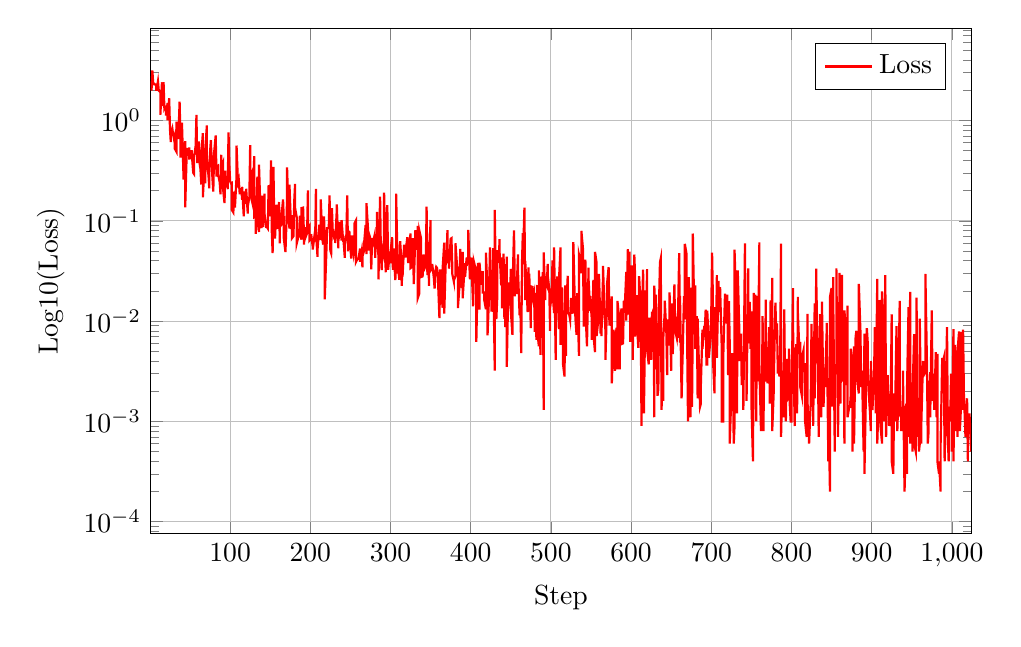
\begin{tikzpicture}
	        		\begin{axis}[
	        			xlabel={Step},
	        			ylabel={Log10(Loss)},
	        			legend pos=north east,
	        			xmin=1, xmax=1024,
	        			grid=major,
	        			width=12cm,
	        			height=8cm,
	        			ymode=log,
	        			log basis y=10,
	        			]

	        			\addplot[
	        			color=red,
	        			mark=none,
	        			thick
	        			] coordinates {
	        				(1,2.4529)
	        				(2,1.9934)
	        				(3,3.1641)
	        				(4,2.3863)
	        				(4,2.3078)
	        				(6,2.2954)
	        				(6,2.3045)
	        				(8,2.2383)
	        				(8,1.9795)
	        				(10,2.4614)
	        				(11,1.9916)
	        				(12,1.9498)
	        				(13,1.9572)
	        				(13,1.1398)
	        				(15,2.4051)
	        				(15,1.3966)
	        				(17,2.4071)
	        				(18,1.3256)
	        				(19,1.3794)
	        				(20,1.3614)
	        				(20,1.1208)
	        				(22,1.4971)
	        				(22,1.0041)
	        				(24,1.6657)
	        				(25,0.822)
	        				(26,0.6082)
	        				(26,0.7115)
	        				(28,0.8243)
	        				(29,0.7174)
	        				(30,0.6531)
	        				(31,0.7033)
	        				(31,0.5239)
	        				(33,0.4896)
	        				(33,0.9744)
	        				(35,0.6529)
	        				(36,0.8837)
	        				(37,1.5431)
	        				(38,0.6987)
	        				(38,0.4275)
	        				(40,0.9518)
	        				(40,0.9031)
	        				(42,0.2577)
	        				(43,0.517)
	        				(44,0.6218)
	        				(44,0.1361)
	        				(46,0.5337)
	        				(46,0.477)
	        				(48,0.4569)
	        				(49,0.5393)
	        				(49,0.4188)
	        				(51,0.4195)
	        				(52,0.5045)
	        				(53,0.3815)
	        				(54,0.3007)
	        				(55,0.2926)
	        				(55,0.4309)
	        				(57,0.5578)
	        				(58,1.1373)
	        				(59,0.3758)
	        				(59,0.3984)
	        				(61,0.6192)
	        				(62,0.3701)
	        				(63,0.3292)
	        				(64,0.2303)
	        				(64,0.4474)
	        				(66,0.7487)
	        				(66,0.1717)
	        				(68,0.3512)
	        				(69,0.2364)
	        				(69,0.5168)
	        				(71,0.8925)
	        				(71,0.3878)
	        				(73,0.2851)
	        				(74,0.2109)
	        				(74,0.3656)
	        				(76,0.6384)
	        				(77,0.3685)
	        				(78,0.2615)
	        				(79,0.1956)
	        				(80,0.4796)
	        				(80,0.4728)
	        				(82,0.7087)
	        				(83,0.2754)
	        				(84,0.3486)
	        				(85,0.3538)
	        				(85,0.2905)
	        				(87,0.2431)
	        				(88,0.1838)
	        				(89,0.4555)
	        				(89,0.3387)
	        				(91,0.376)
	        				(91,0.2174)
	        				(93,0.1504)
	        				(94,0.3163)
	        				(94,0.2766)
	        				(96,0.2711)
	        				(97,0.2066)
	        				(98,0.7607)
	        				(99,0.3656)
	        				(100,0.247)
	        				(101,0.2375)
	        				(102,0.2392)
	        				(102,0.1289)
	        				(104,0.1213)
	        				(105,0.1957)
	        				(106,0.1604)
	        				(106,0.1355)
	        				(108,0.2749)
	        				(108,0.563)
	        				(110,0.2142)
	        				(111,0.2406)
	        				(112,0.184)
	        				(112,0.1971)
	        				(114,0.2068)
	        				(115,0.1623)
	        				(115,0.2167)
	        				(117,0.1107)
	        				(118,0.1959)
	        				(119,0.1475)
	        				(120,0.207)
	        				(120,0.2086)
	        				(122,0.118)
	        				(122,0.1396)
	        				(124,0.1717)
	        				(125,0.5669)
	        				(125,0.2662)
	        				(127,0.2963)
	        				(127,0.1611)
	        				(129,0.1368)
	        				(130,0.4402)
	        				(130,0.1087)
	        				(132,0.1116)
	        				(132,0.0741)
	        				(134,0.2752)
	        				(134,0.1238)
	        				(136,0.0774)
	        				(136,0.3626)
	        				(138,0.1119)
	        				(139,0.0844)
	        				(140,0.1786)
	        				(141,0.0863)
	        				(141,0.0893)
	        				(143,0.1867)
	        				(143,0.1157)
	        				(145,0.085)
	        				(145,0.0889)
	        				(147,0.0839)
	        				(148,0.2261)
	        				(149,0.1109)
	        				(150,0.139)
	        				(151,0.4012)
	        				(152,0.0774)
	        				(153,0.0476)
	        				(154,0.3458)
	        				(155,0.1015)
	        				(156,0.0665)
	        				(157,0.1113)
	        				(158,0.1446)
	        				(159,0.0849)
	        				(160,0.0854)
	        				(161,0.1539)
	        				(162,0.0596)
	        				(162,0.0867)
	        				(164,0.0919)
	        				(164,0.1082)
	        				(166,0.1636)
	        				(167,0.0972)
	        				(167,0.0664)
	        				(169,0.0488)
	        				(170,0.0838)
	        				(171,0.1646)
	        				(171,0.3407)
	        				(173,0.1032)
	        				(174,0.0836)
	        				(174,0.2294)
	        				(176,0.0826)
	        				(177,0.114)
	        				(177,0.0669)
	        				(179,0.0704)
	        				(180,0.1593)
	        				(181,0.2335)
	        				(181,0.1343)
	        				(183,0.1091)
	        				(183,0.0592)
	        				(185,0.0687)
	        				(186,0.0716)
	        				(187,0.1124)
	        				(188,0.0712)
	        				(189,0.0649)
	        				(189,0.1339)
	        				(191,0.1353)
	        				(192,0.0759)
	        				(192,0.058)
	        				(194,0.0866)
	        				(194,0.0683)
	        				(196,0.0754)
	        				(197,0.2008)
	        				(197,0.0838)
	        				(199,0.0887)
	        				(199,0.0638)
	        				(201,0.0668)
	        				(201,0.0737)
	        				(203,0.0548)
	        				(203,0.0517)
	        				(205,0.069)
	        				(206,0.0621)
	        				(207,0.2079)
	        				(207,0.0779)
	        				(209,0.0437)
	        				(209,0.0518)
	        				(211,0.084)
	        				(211,0.0917)
	        				(213,0.0644)
	        				(213,0.1634)
	        				(215,0.0658)
	        				(216,0.0579)
	        				(217,0.1104)
	        				(218,0.0702)
	        				(218,0.0165)
	        				(220,0.0485)
	        				(221,0.0838)
	        				(221,0.0844)
	        				(223,0.0847)
	        				(224,0.1794)
	        				(225,0.0503)
	        				(226,0.0475)
	        				(227,0.1334)
	        				(228,0.0723)
	        				(228,0.0829)
	        				(230,0.0663)
	        				(231,0.0661)
	        				(231,0.0601)
	        				(233,0.1283)
	        				(233,0.1459)
	        				(235,0.0532)
	        				(235,0.0636)
	        				(237,0.0821)
	        				(237,0.0974)
	        				(239,0.0637)
	        				(239,0.1017)
	        				(241,0.0617)
	        				(241,0.0712)
	        				(243,0.0428)
	        				(243,0.0578)
	        				(245,0.0732)
	        				(246,0.179)
	        				(247,0.0497)
	        				(247,0.0793)
	        				(249,0.0768)
	        				(249,0.0714)
	        				(251,0.0421)
	        				(252,0.0714)
	        				(252,0.0608)
	        				(254,0.0467)
	        				(255,0.0545)
	        				(255,0.0942)
	        				(257,0.1011)
	        				(257,0.0389)
	        				(259,0.0419)
	        				(260,0.0421)
	        				(260,0.0409)
	        				(262,0.0529)
	        				(262,0.039)
	        				(264,0.0492)
	        				(265,0.0343)
	        				(265,0.0442)
	        				(267,0.0503)
	        				(267,0.0587)
	        				(269,0.091)
	        				(270,0.0466)
	        				(270,0.1498)
	        				(272,0.0816)
	        				(273,0.0504)
	        				(273,0.0749)
	        				(275,0.0662)
	        				(276,0.0328)
	        				(277,0.0655)
	        				(278,0.0659)
	        				(278,0.0598)
	        				(280,0.0707)
	        				(281,0.0427)
	        				(281,0.0471)
	        				(283,0.0738)
	        				(283,0.123)
	        				(285,0.0423)
	        				(285,0.026)
	        				(287,0.1737)
	        				(288,0.0469)
	        				(289,0.0323)
	        				(289,0.055)
	        				(291,0.0466)
	        				(292,0.0714)
	        				(292,0.1913)
	        				(294,0.0307)
	        				(294,0.0378)
	        				(296,0.1433)
	        				(297,0.034)
	        				(297,0.0325)
	        				(299,0.0472)
	        				(300,0.0376)
	        				(300,0.0484)
	        				(302,0.0685)
	        				(303,0.0325)
	        				(304,0.053)
	        				(304,0.0487)
	        				(306,0.0257)
	        				(307,0.0374)
	        				(307,0.1863)
	        				(309,0.0297)
	        				(309,0.0365)
	        				(311,0.0258)
	        				(312,0.0628)
	        				(313,0.0474)
	        				(314,0.0225)
	        				(315,0.0418)
	        				(315,0.0278)
	        				(317,0.0579)
	        				(317,0.0534)
	        				(319,0.0431)
	        				(319,0.0513)
	        				(321,0.0685)
	        				(322,0.0379)
	        				(323,0.064)
	        				(323,0.0575)
	        				(325,0.0747)
	        				(325,0.0338)
	        				(327,0.0348)
	        				(328,0.067)
	        				(329,0.0234)
	        				(330,0.0407)
	        				(331,0.0805)
	        				(332,0.0589)
	        				(333,0.0515)
	        				(334,0.0889)
	        				(334,0.017)
	        				(336,0.019)
	        				(336,0.0794)
	        				(338,0.0672)
	        				(338,0.0275)
	        				(340,0.0279)
	        				(341,0.0365)
	        				(341,0.0461)
	        				(343,0.0343)
	        				(344,0.0358)
	        				(345,0.1388)
	        				(346,0.0288)
	        				(347,0.0612)
	        				(348,0.0224)
	        				(348,0.0374)
	        				(350,0.1018)
	        				(350,0.0321)
	        				(352,0.0342)
	        				(352,0.0371)
	        				(354,0.0272)
	        				(355,0.0211)
	        				(356,0.0312)
	        				(357,0.0347)
	        				(358,0.0339)
	        				(359,0.0298)
	        				(359,0.0287)
	        				(361,0.0107)
	        				(362,0.0327)
	        				(363,0.0182)
	        				(364,0.0169)
	        				(365,0.0136)
	        				(365,0.0334)
	        				(367,0.0606)
	        				(367,0.0119)
	        				(369,0.0423)
	        				(370,0.0433)
	        				(371,0.0807)
	        				(371,0.0378)
	        				(373,0.0458)
	        				(373,0.0333)
	        				(375,0.0662)
	        				(376,0.067)
	        				(377,0.0358)
	        				(377,0.0296)
	        				(379,0.0248)
	        				(379,0.0254)
	        				(381,0.0281)
	        				(381,0.0597)
	        				(383,0.0353)
	        				(384,0.0336)
	        				(384,0.0135)
	        				(386,0.0223)
	        				(387,0.0526)
	        				(387,0.0393)
	        				(389,0.0214)
	        				(390,0.0489)
	        				(390,0.0169)
	        				(392,0.0308)
	        				(393,0.0378)
	        				(393,0.0277)
	        				(395,0.0432)
	        				(395,0.0357)
	        				(397,0.0445)
	        				(397,0.0812)
	        				(399,0.0261)
	        				(399,0.0311)
	        				(401,0.043)
	        				(401,0.0373)
	        				(403,0.014)
	        				(404,0.031)
	        				(404,0.039)
	        				(406,0.0334)
	        				(407,0.0244)
	        				(407,0.0062)
	        				(409,0.0381)
	        				(409,0.0234)
	        				(411,0.013)
	        				(411,0.0382)
	        				(413,0.023)
	        				(413,0.0237)
	        				(415,0.0315)
	        				(415,0.0193)
	        				(417,0.0193)
	        				(417,0.0161)
	        				(419,0.0131)
	        				(419,0.0482)
	        				(421,0.0193)
	        				(421,0.0072)
	        				(423,0.0189)
	        				(424,0.0543)
	        				(424,0.0168)
	        				(426,0.0279)
	        				(426,0.0124)
	        				(428,0.0533)
	        				(428,0.0405)
	        				(430,0.0032)
	        				(430,0.1284)
	        				(432,0.0105)
	        				(433,0.0165)
	        				(433,0.051)
	        				(435,0.0381)
	        				(436,0.0657)
	        				(436,0.0489)
	        				(438,0.0227)
	        				(439,0.0432)
	        				(439,0.0134)
	        				(441,0.0471)
	        				(442,0.0105)
	        				(443,0.037)
	        				(443,0.0087)
	        				(445,0.044)
	        				(445,0.0035)
	        				(447,0.0243)
	        				(448,0.0159)
	        				(449,0.015)
	        				(450,0.0331)
	        				(450,0.0128)
	        				(452,0.0073)
	        				(452,0.0175)
	        				(454,0.0804)
	        				(455,0.0209)
	        				(455,0.0177)
	        				(457,0.0275)
	        				(457,0.0187)
	        				(459,0.0462)
	        				(459,0.0312)
	        				(461,0.0114)
	        				(462,0.0137)
	        				(463,0.0048)
	        				(464,0.0389)
	        				(465,0.0755)
	        				(465,0.0367)
	        				(467,0.1351)
	        				(468,0.0162)
	        				(468,0.0397)
	        				(470,0.0192)
	        				(471,0.0123)
	        				(472,0.0343)
	        				(473,0.0174)
	        				(473,0.0298)
	        				(475,0.0085)
	        				(475,0.0222)
	        				(477,0.0219)
	        				(477,0.0166)
	        				(479,0.0193)
	        				(480,0.0078)
	        				(480,0.0191)
	        				(482,0.0065)
	        				(483,0.0229)
	        				(483,0.0081)
	        				(485,0.0056)
	        				(485,0.032)
	        				(487,0.0046)
	        				(488,0.0278)
	        				(489,0.0235)
	        				(490,0.0308)
	        				(491,0.0013)
	        				(491,0.0485)
	        				(493,0.0162)
	        				(493,0.0266)
	        				(495,0.0233)
	        				(496,0.0372)
	        				(496,0.029)
	        				(498,0.0208)
	        				(499,0.008)
	        				(499,0.0136)
	        				(501,0.0178)
	        				(502,0.0404)
	        				(502,0.0197)
	        				(504,0.012)
	        				(504,0.0544)
	        				(506,0.0041)
	        				(506,0.0166)
	        				(508,0.0279)
	        				(508,0.0243)
	        				(510,0.0083)
	        				(510,0.0247)
	        				(512,0.0542)
	        				(512,0.0058)
	        				(514,0.0217)
	        				(515,0.0078)
	        				(515,0.0038)
	        				(517,0.0028)
	        				(518,0.0227)
	        				(519,0.0045)
	        				(519,0.0122)
	        				(521,0.0283)
	        				(521,0.0123)
	        				(523,0.0115)
	        				(524,0.0103)
	        				(525,0.017)
	        				(526,0.0147)
	        				(526,0.0121)
	        				(528,0.0122)
	        				(528,0.0612)
	        				(530,0.0132)
	        				(531,0.0095)
	        				(532,0.0073)
	        				(533,0.0113)
	        				(533,0.019)
	        				(535,0.0045)
	        				(535,0.046)
	        				(537,0.0391)
	        				(538,0.03)
	        				(538,0.0795)
	        				(540,0.0525)
	        				(541,0.0088)
	        				(542,0.0367)
	        				(543,0.0409)
	        				(544,0.0087)
	        				(545,0.0056)
	        				(545,0.0058)
	        				(547,0.0341)
	        				(547,0.0259)
	        				(549,0.0126)
	        				(549,0.0177)
	        				(551,0.0104)
	        				(551,0.0065)
	        				(553,0.0258)
	        				(553,0.0075)
	        				(555,0.0049)
	        				(555,0.049)
	        				(557,0.0381)
	        				(557,0.0071)
	        				(559,0.0101)
	        				(560,0.0217)
	        				(560,0.0296)
	        				(562,0.0075)
	        				(563,0.014)
	        				(563,0.0071)
	        				(565,0.0279)
	        				(565,0.0355)
	        				(567,0.0114)
	        				(568,0.0081)
	        				(568,0.0041)
	        				(570,0.015)
	        				(570,0.0234)
	        				(572,0.0345)
	        				(573,0.009)
	        				(574,0.0121)
	        				(575,0.0144)
	        				(576,0.0176)
	        				(576,0.0024)
	        				(578,0.0082)
	        				(579,0.0039)
	        				(580,0.0032)
	        				(580,0.0067)
	        				(582,0.0086)
	        				(583,0.0033)
	        				(583,0.0159)
	        				(585,0.0109)
	        				(586,0.0033)
	        				(586,0.0087)
	        				(588,0.0134)
	        				(588,0.0059)
	        				(590,0.006)
	        				(591,0.016)
	        				(592,0.0121)
	        				(592,0.013)
	        				(594,0.0309)
	        				(594,0.0101)
	        				(596,0.0522)
	        				(596,0.0116)
	        				(598,0.0493)
	        				(599,0.0062)
	        				(600,0.0082)
	        				(601,0.0359)
	        				(602,0.0199)
	        				(602,0.0041)
	        				(604,0.0461)
	        				(605,0.0283)
	        				(605,0.007)
	        				(607,0.0181)
	        				(608,0.0077)
	        				(609,0.0054)
	        				(610,0.0182)
	        				(610,0.0281)
	        				(612,0.0142)
	        				(613,0.0009)
	        				(613,0.0076)
	        				(615,0.0326)
	        				(616,0.0025)
	        				(616,0.0012)
	        				(618,0.0202)
	        				(619,0.0149)
	        				(620,0.0329)
	        				(620,0.0052)
	        				(622,0.0037)
	        				(623,0.0108)
	        				(623,0.0098)
	        				(625,0.0041)
	        				(626,0.0124)
	        				(626,0.0098)
	        				(628,0.0133)
	        				(629,0.0011)
	        				(629,0.0226)
	        				(631,0.0033)
	        				(631,0.0184)
	        				(633,0.0018)
	        				(634,0.0021)
	        				(635,0.0168)
	        				(636,0.0384)
	        				(637,0.042)
	        				(638,0.0013)
	        				(639,0.003)
	        				(640,0.0016)
	        				(640,0.0064)
	        				(642,0.0126)
	        				(642,0.016)
	        				(644,0.0076)
	        				(645,0.0029)
	        				(645,0.0104)
	        				(647,0.0068)
	        				(648,0.0057)
	        				(648,0.0193)
	        				(650,0.0032)
	        				(651,0.015)
	        				(652,0.0132)
	        				(652,0.0047)
	        				(654,0.0232)
	        				(655,0.0081)
	        				(656,0.0074)
	        				(657,0.0068)
	        				(658,0.0111)
	        				(658,0.0068)
	        				(660,0.0476)
	        				(661,0.0061)
	        				(661,0.0178)
	        				(663,0.0017)
	        				(664,0.0039)
	        				(664,0.0037)
	        				(666,0.0177)
	        				(667,0.0104)
	        				(667,0.0589)
	        				(669,0.0474)
	        				(669,0.0322)
	        				(671,0.001)
	        				(672,0.002)
	        				(672,0.0274)
	        				(674,0.0011)
	        				(674,0.0215)
	        				(676,0.0014)
	        				(677,0.0123)
	        				(677,0.0747)
	        				(679,0.0095)
	        				(680,0.0227)
	        				(680,0.0053)
	        				(682,0.0112)
	        				(683,0.0017)
	        				(683,0.0106)
	        				(685,0.0028)
	        				(686,0.0014)
	        				(687,0.0015)
	        				(687,0.0023)
	        				(689,0.0082)
	        				(689,0.0053)
	        				(691,0.0084)
	        				(692,0.0082)
	        				(693,0.013)
	        				(694,0.0037)
	        				(695,0.0037)
	        				(695,0.0127)
	        				(697,0.0054)
	        				(697,0.0043)
	        				(699,0.0068)
	        				(700,0.0122)
	        				(701,0.0482)
	        				(702,0.017)
	        				(702,0.0044)
	        				(704,0.0019)
	        				(705,0.0138)
	        				(706,0.0078)
	        				(707,0.0288)
	        				(707,0.0043)
	        				(709,0.0251)
	        				(710,0.0123)
	        				(711,0.0173)
	        				(711,0.0218)
	        				(713,0.0056)
	        				(713,0.001)
	        				(715,0.001)
	        				(715,0.0046)
	        				(717,0.0174)
	        				(717,0.0188)
	        				(719,0.0095)
	        				(720,0.0184)
	        				(721,0.0029)
	        				(722,0.0158)
	        				(723,0.006)
	        				(723,0.0006)
	        				(725,0.0018)
	        				(726,0.0048)
	        				(727,0.003)
	        				(728,0.0006)
	        				(729,0.0009)
	        				(729,0.0516)
	        				(731,0.0151)
	        				(732,0.0012)
	        				(733,0.0321)
	        				(734,0.0158)
	        				(735,0.0079)
	        				(735,0.004)
	        				(737,0.0075)
	        				(738,0.0023)
	        				(739,0.0028)
	        				(740,0.0049)
	        				(740,0.0013)
	        				(742,0.0596)
	        				(742,0.0053)
	        				(744,0.0038)
	        				(744,0.0016)
	        				(746,0.0335)
	        				(746,0.006)
	        				(748,0.0155)
	        				(749,0.0053)
	        				(750,0.0125)
	        				(750,0.0016)
	        				(752,0.0004)
	        				(753,0.0191)
	        				(753,0.0025)
	        				(755,0.0184)
	        				(756,0.001)
	        				(757,0.0178)
	        				(758,0.0025)
	        				(759,0.0138)
	        				(760,0.0608)
	        				(760,0.0036)
	        				(762,0.0008)
	        				(763,0.0013)
	        				(764,0.0112)
	        				(765,0.0008)
	        				(766,0.0037)
	        				(767,0.0029)
	        				(768,0.0164)
	        				(768,0.0025)
	        				(770,0.0055)
	        				(770,0.0024)
	        				(772,0.0087)
	        				(773,0.0015)
	        				(774,0.0161)
	        				(775,0.002)
	        				(776,0.027)
	        				(776,0.0008)
	        				(778,0.0021)
	        				(778,0.0027)
	        				(780,0.0153)
	        				(781,0.0071)
	        				(782,0.0095)
	        				(783,0.003)
	        				(783,0.0042)
	        				(785,0.0028)
	        				(786,0.005)
	        				(787,0.0593)
	        				(787,0.0007)
	        				(789,0.0032)
	        				(790,0.0011)
	        				(791,0.0131)
	        				(792,0.0021)
	        				(793,0.001)
	        				(794,0.0042)
	        				(794,0.0016)
	        				(796,0.0017)
	        				(797,0.0053)
	        				(798,0.0014)
	        				(799,0.001)
	        				(800,0.001)
	        				(800,0.0014)
	        				(802,0.0213)
	        				(802,0.0085)
	        				(804,0.0009)
	        				(805,0.0043)
	        				(806,0.0059)
	        				(807,0.0012)
	        				(808,0.0174)
	        				(808,0.012)
	        				(810,0.0047)
	        				(811,0.0062)
	        				(811,0.0022)
	        				(813,0.0018)
	        				(814,0.0047)
	        				(815,0.0051)
	        				(815,0.0031)
	        				(817,0.0038)
	        				(817,0.001)
	        				(819,0.0007)
	        				(820,0.0118)
	        				(820,0.0016)
	        				(822,0.0006)
	        				(823,0.001)
	        				(824,0.0015)
	        				(825,0.0094)
	        				(826,0.0014)
	        				(827,0.0048)
	        				(827,0.0009)
	        				(829,0.015)
	        				(829,0.0017)
	        				(831,0.0333)
	        				(831,0.0234)
	        				(833,0.0035)
	        				(834,0.0007)
	        				(834,0.0019)
	        				(836,0.0117)
	        				(837,0.0011)
	        				(838,0.0024)
	        				(838,0.0156)
	        				(840,0.0014)
	        				(841,0.0027)
	        				(842,0.0022)
	        				(843,0.0048)
	        				(844,0.0083)
	        				(844,0.0096)
	        				(846,0.0004)
	        				(846,0.0017)
	        				(848,0.0002)
	        				(848,0.0173)
	        				(850,0.0213)
	        				(851,0.0014)
	        				(852,0.0274)
	        				(852,0.0195)
	        				(854,0.0005)
	        				(854,0.0029)
	        				(856,0.0037)
	        				(856,0.0336)
	        				(858,0.0007)
	        				(859,0.0028)
	        				(860,0.0303)
	        				(861,0.0119)
	        				(861,0.0015)
	        				(863,0.0289)
	        				(863,0.0025)
	        				(865,0.0096)
	        				(866,0.0006)
	        				(866,0.0128)
	        				(868,0.0078)
	        				(869,0.0023)
	        				(870,0.0143)
	        				(870,0.0011)
	        				(872,0.0014)
	        				(873,0.0014)
	        				(874,0.0019)
	        				(874,0.0053)
	        				(876,0.0037)
	        				(876,0.0005)
	        				(878,0.0056)
	        				(878,0.0006)
	        				(880,0.007)
	        				(881,0.008)
	        				(881,0.0035)
	        				(883,0.0022)
	        				(884,0.0019)
	        				(884,0.0235)
	        				(886,0.0079)
	        				(887,0.0022)
	        				(888,0.0031)
	        				(888,0.0032)
	        				(890,0.0005)
	        				(891,0.0075)
	        				(891,0.0003)
	        				(893,0.0022)
	        				(894,0.0085)
	        				(895,0.0063)
	        				(895,0.0038)
	        				(897,0.0016)
	        				(898,0.0012)
	        				(899,0.0008)
	        				(899,0.004)
	        				(901,0.0013)
	        				(901,0.0013)
	        				(903,0.003)
	        				(904,0.0087)
	        				(905,0.0056)
	        				(905,0.0012)
	        				(907,0.0263)
	        				(907,0.0006)
	        				(909,0.002)
	        				(910,0.0162)
	        				(911,0.0139)
	        				(911,0.0009)
	        				(913,0.0006)
	        				(913,0.0198)
	        				(915,0.0084)
	        				(916,0.001)
	        				(917,0.0288)
	        				(918,0.0008)
	        				(918,0.0007)
	        				(920,0.0029)
	        				(920,0.0017)
	        				(922,0.0018)
	        				(922,0.0009)
	        				(924,0.0024)
	        				(925,0.0117)
	        				(925,0.0004)
	        				(927,0.0003)
	        				(928,0.0019)
	        				(929,0.0014)
	        				(929,0.001)
	        				(931,0.0089)
	        				(932,0.0008)
	        				(933,0.0015)
	        				(933,0.0018)
	        				(935,0.0159)
	        				(935,0.0012)
	        				(937,0.0013)
	        				(937,0.0008)
	        				(939,0.0019)
	        				(939,0.0032)
	        				(941,0.0002)
	        				(942,0.0004)
	        				(943,0.0015)
	        				(944,0.0003)
	        				(944,0.0019)
	        				(946,0.0138)
	        				(947,0.0007)
	        				(948,0.0196)
	        				(948,0.0006)
	        				(950,0.0013)
	        				(951,0.0005)
	        				(951,0.0019)
	        				(953,0.0074)
	        				(953,0.0006)
	        				(955,0.0005)
	        				(956,0.0171)
	        				(957,0.0007)
	        				(958,0.0012)
	        				(959,0.0005)
	        				(960,0.0006)
	        				(960,0.0106)
	        				(962,0.0006)
	        				(962,0.001)
	        				(964,0.004)
	        				(964,0.0028)
	        				(966,0.003)
	        				(967,0.0032)
	        				(967,0.0296)
	        				(969,0.0036)
	        				(970,0.0006)
	        				(971,0.0008)
	        				(971,0.0012)
	        				(973,0.0031)
	        				(973,0.0011)
	        				(975,0.0128)
	        				(976,0.0016)
	        				(977,0.003)
	        				(978,0.0014)
	        				(978,0.0013)
	        				(980,0.0049)
	        				(981,0.0011)
	        				(982,0.0047)
	        				(982,0.0004)
	        				(984,0.0003)
	        				(984,0.0004)
	        				(986,0.0002)
	        				(986,0.0006)
	        				(988,0.0043)
	        				(988,0.0037)
	        				(990,0.0043)
	        				(991,0.0004)
	        				(992,0.001)
	        				(992,0.0014)
	        				(994,0.0087)
	        				(995,0.0007)
	        				(996,0.0004)
	        				(996,0.0014)
	        				(998,0.001)
	        				(999,0.003)
	        				(1000,0.0015)
	        				(1000,0.0005)
	        				(1002,0.0083)
	        				(1002,0.0004)
	        				(1004,0.0058)
	        				(1004,0.0008)
	        				(1006,0.0033)
	        				(1007,0.0007)
	        				(1007,0.0049)
	        				(1009,0.0079)
	        				(1010,0.0008)
	        				(1011,0.0012)
	        				(1011,0.0078)
	        				(1013,0.0013)
	        				(1014,0.0082)
	        				(1015,0.002)
	        				(1015,0.0019)
	        				(1017,0.0007)
	        				(1017,0.0007)
	        				(1019,0.0017)
	        				(1020,0.0004)
	        				(1020,0.001)
	        				(1022,0.001)
	        				(1022,0.0012)
	        				(1024,0.0005)
	        			};
	        			\addlegendentry{Loss}

	        		\end{axis}
	        	\end{tikzpicture}
	        	\caption{Log10(Loss) Over Training Steps}
	        	\label{fig:log_loss}
	        \end{figure}


	\chapter{Results \& Discussion}\label{ch:results-and-discussion}
		\section{Example Input}\label{sec:example-input}
	        As an example, we consider the following input:
	        \begin{itquote}
				Jetzt ist ja Klima ein grosses Thema.
				Sie haben sich bisher nicht gross geäussert.
				Jetzt ist eine Strategie in Zürich rausgekommen, man will die rot-grüne Klimapanik bekämpfen.
				Wie stehen Sie jetzt zu diesem Thema?
				Wie stehen Sie zu diesen Demonstrationen von all diesen Kindern und Schülern, die wöchentlich auf die Strasse gehen?
				Die, die auf die Strasse gehen und sagen, wir sind für ein gesundes Klima, da kann ich niemandem dagegen sein.
				Das ist ja schön, wenn sie das machen.
				Aber was dahinter steht, politisch bei den Grünen, das sind Sachen, die ganz verwerflich sind.
				Die wollen jetzt das lösen, mehr Eingriffe vom Staat, mehr Steuern, Abgaben, Gebühren, 20 ApB fürs Benzin, Heizkosten bis zu 1400 Franken pro Haushalt.
				Dann, was wir sollen essen und nicht sollen essen und wie wir sollen essen und wie wir sollen leben und wohnen und wie gross die Wohnungen sind, das hört nicht mehr auf.
				Gegen das sind wir massiv.
				Das ist ein Eingriff in die Freiheit und bringt dem Klima schlussendlich gar nichts.
				Was würde Ihrer Meinung nach etwas bringen, um den Klimawandel zu stoppen?
				Weiterfahren mit dem Programm, das wir jetzt haben.
				Wir müssen mal schauen, was wir schon alles haben.
				Wir haben die ganze Gewässerverschmutzung unter Kontrolle.
				Wir haben saubere Gewässer, sagen mir die Fischer, oder?
				Weil wir sogar das Meteowasser reinigen.
				Wir haben Rauchgasreinigung.
				Wir haben beim Auto Abgasvorschriften eingeführt.
				Wir gehen noch weiter mit dem.
				Muss ja technologisch möglich sein.
				Und dann die Innovation nicht vom Staat fördern, sondern schauen, dass die Privaten etwas machen.
				Wer hat ein Elektroauto?
				Wer hat ein Hybrid gemacht?
				Nicht der Staat und auch nicht die Grünen, sondern die Autoindustrie, die Wirtschaft hat das entwickelt.
				Kommt mit dem.
				Ich höre, sie arbeiten schon an den Flugzeugen.
				Sie wollen abgasfreie Flugzeuge.
				Auf der Lärmseite höre ich, das sind doch Massnahmen, die wir treffen müssen.
				Wir treffen sie nicht, weil das Klima sonst kaputt geht, sondern weil wir saubere Luft, reines Wasser, gesunden Boden wollen.
				Das war immer das Programm und bei dem müssen wir bleiben.
				Und dann wird es gut kommen.
				Kann man denn mit einer Klima-Offensive bei der SVP rechnen?
				Weil bisher hat man eher nur gehört, auch gerade von Herr Köppel, die Politik der anderen, die Klimapolitik der anderen, lehnen wir ab.
				Aber einen Vorschlag von ihnen haben wir noch nicht.
				Wir brauchen keine.
				Wir machen schon alles.
				Das habe ich gerade eben gesagt.
				Das müssen wir weiterführen.
				Das ist aber theoretisch nichts machen.
				Diese Strategie hat ja nicht wirklich \ldots
				Nichts falsches machen.
				Sie möchten gerne, dass wir die falschen Massnahmen machen.
				Jetzt wollen wir mehr Lenkungsabgaben.
				Jetzt wollen wir mehr für das Benzin.
				Das haben die in den Städten, die das Tram vor der Tür haben, die können das gut sagen.
				Die Leute der Agglomeration, die in die Stadt möchten, wo Züge und alles verstopft ist.
				Bei der Zuwanderung, die der Hauptgrund ist, machen die nichts.
				Da sind wir in der Offensive.
				Jetzt kommt ja die Begrenzungsinitiative.
			\end{itquote}
	        This is the transcript of the interview with Christoph Blocher, a billionaire and former member of the Swiss Federal Council~\cite{blocher}.
	        It has been published in the Swiss digital newspaper \enquote{Nau.ch}~\cite{baerlocher2019} and was chosen as it has a large overlap with the included test database.
	        Only minor parts are in the training data and the rest is new to the Large Language Model.

	    \section{Output}\label{sec:output}
			\begin{itquote}
				Jetzt ist ja Klima ein grosses Thema.\\
				Sie haben sich bisher nicht gross geäussert.\\
				Jetzt ist eine Strategie in Zürich rausgekommen, man will die rot-grüne Klimapanik bekämpfen.\\
				\\
				  \# Hinweis: Eine Abnahme des Autoverkehrs im Vergleich zu anderen Verkehrsteilnehmer hat positive Auswirkungen auf das lokale Gewerbe.\\
				  \# Hinweis: Mit Ausnahme des Weinbaus ist in der Landwirtschaft wegen der durch den Klimawandel verursachten Trockenheit praktisch überall mit negativen Auswirkungen zu rechnen.\\
				  \# Hinweis: Die BILD-Zeitung verbreitete Lügen über die Berliner Polizistin J.S., welche die BILD später selber als unwahr bestätigte.\\
				Wie stehen Sie jetzt zu diesem Thema?\\
				Wie stehen Sie zu diesen Demonstrationen von all diesen Kindern und Schülern, die wöchentlich auf die Strasse gehen?\\
				Die, die auf die Strasse gehen und sagen, wir sind für ein gesundes Klima, da kann ich niemandem dagegen sein.\\
				\\
				  \# Hinweis: Eine Abnahme des Autoverkehrs im Vergleich zu anderen Verkehrsteilnehmer hat positive Auswirkungen auf das lokale Gewerbe.\\
				  \# Hinweis: Die BILD-Zeitung verbreitete Lügen über die Berliner Polizistin J.S., welche die BILD später selber als unwahr bestätigte.\\
				  \# Hinweis: Ozonlöcher waren eine erhebliche Gefahr für die Umwelt und die menschliche Gesundheit, da sie die schädlichen UV-Strahlen der Sonne direkt auf die Erdoberfläche lassen. Ozonlöcher sind heute keine Probleme mehr, weil die Welt konkret handelte – anders als beim Klimawandel. Im Montreal-Protokoll von 1987 wurden ganze Stoffklassen verboten.\\
				Das ist ja schön, wenn sie das machen.\\
				Aber was dahinter steht, politisch bei den Grünen, das sind Sachen, die ganz verwerflich sind.\\
				Die wollen jetzt das lösen, mehr Eingriffe vom Staat, mehr Steuern, Abgaben, Gebühren, 20 ApB fürs Benzin, Heizkosten bis zu 1400 Franken pro Haushalt.\\
				\\
				  \# Hinweis: Gemäss Parteien, die zu dem politisch-rechten Flügel gezählt werden, ist ``woke'' ein ``umgangssprachlicher Begriff für einen allgemeinen Glauben an systembedingte Ungerechtigkeiten''.\\
				  \# Hinweis: Ozonlöcher waren eine erhebliche Gefahr für die Umwelt und die menschliche Gesundheit, da sie die schädlichen UV-Strahlen der Sonne direkt auf die Erdoberfläche lassen. Ozonlöcher sind heute keine Probleme mehr, weil die Welt konkret handelte – anders als beim Klimawandel. Im Montreal-Protokoll von 1987 wurden ganze Stoffklassen verboten.\\
				Dann, was wir sollen essen und nicht sollen essen und wie wir sollen essen und wie wir sollen leben und wohnen und wie gross die Wohnungen sind, das hört nicht mehr auf.\\
				Gegen das sind wir massiv.\\
				Das ist ein Eingriff in die Freiheit und bringt dem Klima schlussendlich gar nichts.\\
				\\
				  \# Hinweis: In der Wissenschaft herrscht ein starker wissenschaftlicher Konsens darüber, dass ein Klimawandel stattfindet, dieser in diesem Ausmass noch nie ansatzweise existierte, und dass der aktuelle Klimawandel fast ausschliesslich durch menschliche Aktivitäten verursacht wird.\\
				Was würde Ihrer Meinung nach etwas bringen, um den Klimawandel zu stoppen?\\
				Weiterfahren mit dem Programm, das wir jetzt haben.\\
				Wir müssen mal schauen, was wir schon alles haben.\\
				\\
				Wir haben die ganze Gewässerverschmutzung unter Kontrolle.\\
				Wir haben saubere Gewässer, sagen mir die Fischer, oder?\\
				Weil wir sogar das Meteowasser reinigen.\\
				\\
				Wir haben Rauchgasreinigung.\\
				Wir haben beim Auto Abgasvorschriften eingeführt.\\
				Wir gehen noch weiter mit dem.\\
				\\
				  \# Hinweis: Gemäss Parteien, die zu dem politisch-rechten Flügel gezählt werden, ist ``woke'' ein ``umgangssprachlicher Begriff für einen allgemeinen Glauben an systembedingte Ungerechtigkeiten''.\\
				  \# Hinweis: In der Wissenschaft herrscht ein starker wissenschaftlicher Konsens darüber, dass ein Klimawandel stattfindet, dieser in diesem Ausmass noch nie ansatzweise existierte, und dass der aktuelle Klimawandel fast ausschliesslich durch menschliche Aktivitäten verursacht wird.\\
				  \# Hinweis: Laut dem Seco-Bericht wanderten 2017 nur rund 31'250 Personen aus EU- und EFTA-Ländern ein. Das sind 50 Prozent weniger als noch 2013. Zudem zeigt der Bericht, dass rund die Hälfte aller Personen die 2009 in die Schweiz kamen, wieder ausgereist sind.\\
				Muss ja technologisch möglich sein.\\
				Und dann die Innovation nicht vom Staat fördern, sondern schauen, dass die Privaten etwas machen.\\
				Wer hat ein Elektroauto?\\
				\\
				  \# Hinweis: In der Wissenschaft herrscht ein starker wissenschaftlicher Konsens darüber, dass ein Klimawandel stattfindet, dieser in diesem Ausmass noch nie ansatzweise existierte, und dass der aktuelle Klimawandel fast ausschliesslich durch menschliche Aktivitäten verursacht wird.\\
				Wer hat ein Hybrid gemacht?\\
				Nicht der Staat und auch nicht die Grünen, sondern die Autoindustrie, die Wirtschaft hat das entwickelt.\\
				Kommt mit dem.\\
				\\
				  \# Hinweis: Eine Abnahme des Autoverkehrs im Vergleich zu anderen Verkehrsteilnehmer hat positive Auswirkungen auf das lokale Gewerbe.\\
				  \# Hinweis: In der Wissenschaft herrscht ein starker wissenschaftlicher Konsens darüber, dass ein Klimawandel stattfindet, dieser in diesem Ausmass noch nie ansatzweise existierte, und dass der aktuelle Klimawandel fast ausschliesslich durch menschliche Aktivitäten verursacht wird.\\
				  \# Hinweis: Die BILD-Zeitung verbreitete Lügen über die Berliner Polizistin J.S., welche die BILD später selber als unwahr bestätigte.\\
				Ich höre, sie arbeiten schon an den Flugzeugen.\\
				Sie wollen abgasfreie Flugzeuge.\\
				Auf der Lärmseite höre ich, das sind doch Massnahmen, die wir treffen müssen.\\
				\\
				  \# Hinweis: Gemäss Parteien, die zu dem politisch-rechten Flügel gezählt werden, ist ``woke'' ein ``umgangssprachlicher Begriff für einen allgemeinen Glauben an systembedingte Ungerechtigkeiten''.\\
				  \# Hinweis: Eine Abnahme des Autoverkehrs im Vergleich zu anderen Verkehrsteilnehmer hat positive Auswirkungen auf das lokale Gewerbe.\\
				  \# Hinweis: In der Wissenschaft herrscht ein starker wissenschaftlicher Konsens darüber, dass ein Klimawandel stattfindet, dieser in diesem Ausmass noch nie ansatzweise existierte, und dass der aktuelle Klimawandel fast ausschliesslich durch menschliche Aktivitäten verursacht wird.\\
				Wir treffen sie nicht, weil das Klima sonst kaputt geht, sondern weil wir saubere Luft, reines Wasser, gesunden Boden wollen.\\
				Das war immer das Programm und bei dem müssen wir bleiben.\\
				Und dann wird es gut kommen.\\
				\\
				Kann man denn mit einer Klima-Offensive bei der SVP rechnen?\\
				Weil bisher hat man eher nur gehört, auch gerade von Herr Köppel, die Politik der anderen, die Klimapolitik der anderen, lehnen wir ab.\\
				Aber einen Vorschlag von ihnen haben wir noch nicht.\\
				\\
				Wir brauchen keine.\\
				Wir machen schon alles.\\
				Das habe ich gerade eben gesagt.\\
				\\
				Das müssen wir weiterführen.\\
				Das ist aber theoretisch nichts machen.\\
				Diese Strategie hat ja nicht wirklich \ldots\\
				\\
				Nichts falsches machen.\\
				Sie möchten gerne, dass wir die falschen Massnahmen machen.\\
				Jetzt wollen wir mehr Lenkungsabgaben.\\
				\\
				Jetzt wollen wir mehr für das Benzin.\\
				Das haben die in den Städten, die das Tram vor der Tür haben, die können das gut sagen.\\
				Die Leute der Agglomeration, die in die Stadt möchten, wo Züge und alles verstopft ist.\\
				\\
				Die Leute der Agglomeration, die in die Stadt möchten, wo Züge und alles verstopft ist.\\
				Bei der Zuwanderung, die der Hauptgrund ist, machen die nichts.\\
				Da sind wir in der Offensive.
			\end{itquote}

	    \section{Evaluation}\label{sec:evaluation}
			This test shows a need for improvement as well as a promising result.
			Notable is the lack of hallucination of topics thanks to the fine-tuning and the hot-swappable Georgi Gerganov Backus Naur Form~\cite{gbnf}.

			The AI loves to include three specific topics:\enquote{woke} \enquote{Berliner Polizistin J.S.} and \enquote{Autofahrer und lokales Gewerbe}.
			\enquote{woke} is a term with a small token count, likely less affected by the fine-tuning.
			\enquote{Berliner Polizistin J.S.} is overrepresented in the training data.
	        But the frequent false inclusion of \enquote{Autofahrer und lokales Gewerbe} is not explainable.

		\section{Conclusion}\label{sec:conclusion}
			In order to avoid hallucinations and false narratives in Large Language Models, we chose to have a human curated dataset of facts.
	        This creates a lot of up-front work to create a production-ready system.

		    While the current implementation has limitations, the underlying technology choices show potential for future development.
			With continued refinement and expansion, systems like PolitScanner could play an important role in countering misinformation in political discourse and strengthening democratic processes.

	        One major drawback of this implementation is the use of Large Language Models that include Chinese censorship.
	        But this should be easy to fix once the European company MistralAI releases their three-billion-parameter model to the public.
	        
	\printbibliography[heading=bibintoc]
\end{document}
